\documentclass[12pt, a4paper]{article}

%%%%%%%% CREATE DOCUMENT STRUCTURE %%%%%%%%
%% Language and font encodings
\usepackage[english]{babel}
\usepackage[utf8]{inputenc}
\usepackage[T1]{fontenc}

%% Sets page size and margins
\usepackage[a4paper,top=3cm,bottom=2.5cm,left=2cm,right=2cm,marginparwidth=1.75cm]{geometry}

%% Useful packages
\usepackage{amsmath}
\usepackage{amssymb}
\usepackage{graphicx}
\usepackage{tikz}
\usetikzlibrary{arrows.meta,positioning, fit, calc, backgrounds, shapes.geometric}
\usepackage[siunitx,american]{circuitikz}
\usepackage[colorlinks=true, allcolors=blue]{hyperref}
\usepackage{caption}
\usepackage{subcaption}
\usepackage{sectsty}
\usepackage{float}
\usepackage{titling}
\usepackage{booktabs}
\usepackage{longtable}
\usepackage{array}
\usepackage{enumitem}
\usepackage{listings}
\usepackage{fancyhdr}
\usepackage[square,sort,comma,numbers]{natbib}
\usepackage{xcolor}
\definecolor{darkgreen}{rgb}{0.0, 0.4, 0.0}
\usepackage{algorithm}
\usepackage{algpseudocode}
\usepackage{tikz-timing}

%% -- Report identity (used by the running header/footer) --
\newcommand{\projectnumber}{323}
\newcommand{\projectname}{FinWatch: an extensible BLE smartwatch platform}
\newcommand{\submissiondate}{\today}
\newcommand{\repourl}{\url{https://github.com/laserblade41/FinProj}}

\pagestyle{fancy}
\fancyhf{}
\fancyhead[L]{\footnotesize Project number: \projectnumber}
\fancyhead[R]{\footnotesize \submissiondate}
\fancyfoot[L]{\footnotesize Project: \projectname}
\fancyfoot[R]{\footnotesize Page \thepage}
\renewcommand{\headrulewidth}{0.4pt}
\renewcommand{\footrulewidth}{0.4pt}


%% -- C listings style (Appendix A) --
\definecolor{lstkey}{rgb}{0.0,0.0,0.6}
\definecolor{lstcom}{rgb}{0.25,0.5,0.35}
\definecolor{lststr}{rgb}{0.6,0.1,0.1}
\lstdefinestyle{cstyle}{
  language=C,
  basicstyle=\ttfamily\scriptsize,
  keywordstyle=\color{lstkey}\bfseries,
  commentstyle=\color{lstcom}\itshape,
  stringstyle=\color{lststr},
  numbers=left,
  numberstyle=\tiny\color{gray},
  numbersep=6pt,
  breaklines=true,
  breakatwhitespace=true,
  showstringspaces=false,
  tabsize=4,
  frame=single,
  rulecolor=\color{gray},
  captionpos=b,
  columns=fullflexible,
  extendedchars=true,
  inputencoding=utf8,
  % The C sources contain UTF-8 em dashes in comments; map them so listings
  % does not choke on the multi-byte sequence.
  literate={—}{{-{}-}}1 {–}{{-}}1 {’}{{'}}1 {“}{{"}}1 {”}{{"}}1
           {±}{{$\pm$}}1 {²}{{\textasciicircum2}}2 {µ}{{u}}1
           {→}{{-{}>}}2 {≈}{{\textasciitilde}}1,
}
\lstset{style=cstyle}

%%%%%%%% DOCUMENT %%%%%%%%
\begin{document}

%%%% Title Page
\begin{titlepage}
\thispagestyle{empty}

\newcommand{\HRule}{\rule{\linewidth}{0.5mm}}
\center

% University
\textsc{\LARGE Bar-Ilan University}\\[0.6cm]
% Faculty
\textsc{\LARGE Faculty of Engineering}\\[0.6cm]
% Document info
\textsc{\Large Final Project in Computer Engineering}\\[0.2cm]
\textsc{\large Course 83453 \quad$\vert$\quad Project 323}\\[1cm]
\HRule \\[0.8cm]
{\huge \bfseries FinWatch}\\[0.35cm]
{\Large An Extensible BLE Smartwatch Platform with a\\ Modular I\textsuperscript{2}C Expansion Port}\\[0.5cm]
% The Hebrew title required by the template cannot be typeset by pdfLaTeX.
% Either compile with XeLaTeX + polyglossia, or paste the Hebrew title as an
% image here. Placeholder kept visible so it is not forgotten:

\includegraphics[width=0.7\textwidth]{images/hebrew title.png}\\[0.4cm]
\HRule \\[1.5cm]

\large
\emph{Authors:}\\[0.15cm]
Omer Lazaros 325248797\\
Chen Leibov 211800552\\[0.8cm]

\begin{tabular}{r l}
Track: & Hardware design\\
Academic supervisor: & Prof.\ Leonid Yavitz \quad leonid.yavitz@biu.ac.il\\
Project mentor: & David Freud \quad david.freud@mail.huj.ac.il\\
Date of submission: & \submissiondate \ / 
\includegraphics[width=0.18\textwidth]{images/hebrew date.png}\\
Github repository: & \repourl
\end{tabular}\\[1.2cm]

\emph{Submitted as part of the undergraduate requirements}\\
\emph{Faculty of Engineering, Bar-Ilan University}\\[1cm]


\includegraphics[width=0.45\textwidth]{images/logo.png}
\vfill
\end{titlepage}

\newpage
\section*{Abstract}
\addcontentsline{toc}{section}{Abstract}

Wrist-worn wearables have become a general-purpose sensing platform, but nearly
all of them, commercial and open-source alike, are sealed products: the set
of sensors is fixed at manufacture, and adding a new measurement means designing
a new watch.\\\\
This project asks whether a wearable can instead be built as an
\emph{extensible} platform, in which a user or a third party attaches new
hardware to a finished, sealed device and the firmware discovers what it is at
runtime.\\\\
% comment to avoid weird latex spacing
We present \textbf{FinWatch}, a complete custom smartwatch built around the
Nordic Semiconductor nRF5340 dual-core Bluetooth Low Energy SoC, with an
nPM1300 power-management IC providing regulated \SI{1.8}{\volt} and
\SI{3.3}{\volt} rails and Li-Po charging, an STMicroelectronics LSM6DSOX
six-axis IMU, a
\SI{512}{\mega\bit} QSPI NOR flash, and an SPI display with capacitive touch.\\\\
The hardware was designed in KiCad as a four-layer PCB and the firmware was
written for the Zephyr RTOS.\\\\
The distinguishing element is a four-pin pogo
connector carrying \SI{3.3}{\volt}, ground, and an I\textsuperscript{2}C bus
level-shifted from the SoC's \SI{1.8}{\volt} domain, together with the
\textbf{FinWatch Module Protocol (FWMP)}: a self-describing, CRC-protected
descriptor format that lets any compliant I\textsuperscript{2}C module announce
its identity, capabilities, report sizes, and preferred polling rate.\\\\
The host treats every byte from an attached module as untrusted, validating magic
numbers, protocol version, declared lengths, TLV bounds, and a CRC-16 before any
field is used.\\\\
% hello
The firmware comprises roughly 2\,550 lines of C across nine subsystems and was
verified functionally on an nRF5340-DK, including hot-plug enumeration,
input/output report exchange, and six injected-fault cases that exercise every
host-side rejection path.\\\\
The first PCB revision was manufactured and its power
rails verified, but a missing SWD debug header prevented on-board firmware
loading and forced a second revision; the design review that produced that
revision is reported as a result in its own right.\\\\
The outcome is a working wearable platform and a documented expansion contract that a third party can
implement without access to the watch firmware.

\newpage
\section*{Acknowledgments}
\addcontentsline{toc}{section}{Acknowledgments}

We would like to thank our project mentor, David Freud, for his guidance
throughout the design, review, and bring-up of this project, and our academic
supervisor, Prof.\ Leonid Yavitz, for his support and supervision. We also thank
the Faculty of Engineering at Bar-Ilan University for providing the laboratory
facilities and equipment used in this work, and the maintainers of the open
tools this project depends on- KiCad, the Zephyr Project, and the nRF Connect
SDK- whose excellent online courses, documentation and reference designs made a project of this scope
feasible within a single academic year.

\newpage
\tableofcontents
\newpage
%\listoffigures
%\listoftables

\newpage
% =================================================================
\section{Introduction}

\subsection{Background}

A modern smartwatch is, at its core, a microcontroller with a radio, a battery,
a display, and a small collection of sensors, packaged so that it can be worn
continuously.\\\\
Over the past decade this form factor has moved well beyond
telling the time: it is now used for continuous health monitoring, fitness
tracking, industrial telemetry, and as a general-purpose personal sensing
platform.\\\\
What makes the category interesting from an engineering standpoint is
the severity of its constraints.\\\\
The device must fit on a wrist, so board area
and battery capacity are fixed and small; it must run for days on that battery,
so average current consumption is measured in microamperes rather than
milliamperes; it must maintain a wireless link, so a sensitive \SI{2.4}{\giga
\hertz} radio has to coexist on the same substrate as switching regulators and a
display backlight; and it must remain responsive to the user, so the firmware has
to service a display, a touch panel, a sensor, and a radio stack concurrently.\\\\
% placeholder
Each of these constraints pulls against the others. Efficient power conversion
requires switching regulators, which generate the electromagnetic interference
that degrades radio sensitivity.\\\\
Long battery life requires the processor to
sleep as much as possible, which conflicts with a display that must redraw and a
sensor that must be sampled.\\\\
Small board area forces components closer together,
which worsens both thermal behaviour and crosstalk.\\\\
A wearable design is
therefore less an exercise in selecting parts than in negotiating between
mutually hostile requirements, and this negotiation is the substance of the
present project.\\\\
% comment to avoid weird latex spacing
There is a second, less technical constraint that motivates this work
specifically.\\\\
A wearable is a sealed object. Once it is assembled, glued, and
made water-resistant, its sensor complement is frozen for the lifetime of the
product.\\\\
If a user, a researcher, or a workplace needs a measurement the
manufacturer did not anticipate- an environmental gas sensor, an
electrochemical probe, an RFID reader, a specialised medical transducer, the
only available answer is a different watch.\\\\
The cost of that answer is not
merely commercial: it means that every new wrist-worn measurement idea must
re-solve power management, radio, display, mechanical design, and certification
from scratch before it can be tested at all.

\subsection{Literature and market overview}
\label{sec:lit}

Approaches to building wrist-worn devices fall into four broad families.

\paragraph{Closed commercial products.} Devices such as those from the major
consumer vendors are highly optimised for battery life, size, and manufacturing
cost. Their internal buses are inaccessible, their firmware is proprietary, and
their sensor set is fixed. Their measurement quality is also not a settled
matter: an independent validation of four low-cost consumer smartwatches against
indirect calorimetry found substantial and device-dependent error in estimated
energy expenditure~\cite{liu2025}, which is worth keeping in mind whenever a
wrist-worn figure is treated as ground truth. They are excellent products and
useless as platforms.

\paragraph{Open-source wearables.} The PineTime and Bangle.js represent the
open end of the spectrum: both publish schematics and allow user firmware, and
both have active communities. Architecturally they are close to this project-
an nRF52-class SoC, an SPI display, an accelerometer, a Li-Po cell- and their
existence is what makes the hardware side of this project tractable as a student
effort.\\\\
But they are open in the sense of \emph{modifiable firmware}, not
\emph{extensible hardware}. Neither exposes a documented electrical and logical
interface through which a sealed device can acquire new sensing capability
after manufacture.\\\\
Adding a sensor to a PineTime means opening it and soldering
to test pads, at which point water resistance and mechanical integrity are gone.

\paragraph{ZSWatch.}
\label{lit:zswatch}
The closest prior work to this project is ZSWatch, an open-source smartwatch
built on an nRF5340 (as a u-blox NORA-B10 module) running Zephyr, with an
nPM1300 PMIC, a Bosch BMI270 IMU, a Macronix MX25U51245G external flash, and a
$240\times240$ round touch display.\\\\
The convergence with the present design is close enough to be worth stating
plainly: the same SoC, the same RTOS, the same PMIC, the same external flash
part, and, as originally specified, the same IMU.\\\\
This is less coincidence than evidence that the component space for an open Zephyr wearable is narrow, and
that two independent projects arrived at the same defensible answers within it.
ZSWatch is considerably more mature than this project and carries a richer
sensor complement, including barometric, magnetometer, ambient-light and
microphone channels that this design does not have.\\\\
Where the two diverge is expansion. ZSWatch does offer an Extension PCB, but it
plugs into the breakout headers of the separate \emph{WatchDK} development
board rather than into the finished watch, and it is a specific first-party
add-on- heart rate and an audio codec- supported by drivers written for it.
That is expansion in the development-kit sense, the same sense in which the
nRF5340-DK is expandable, and it does not address a sealed device acquiring
capability from hardware its firmware has never seen. ZSWatch's dock is a USB-C
breakout for debugger and UART access rather than a peripheral bus, and no
self-describing descriptor or runtime discovery mechanism is documented for
either interface.

\paragraph{Research prototypes.} A third family exists only in the literature,
and it optimises for a different axis again: energy autonomy. Chen and
Rodriguez-Villegas~\cite{chen2025} describe a battery-free wristband that runs
indefinitely on indoor light by combining solar harvesting with a supercapacitor,
an adaptive sampling policy that spends energy according to what the sensor is
actually seeing, and on-board processing that exists specifically to avoid paying
for radio transmissions.\\\\
Work on the supply side is comparable in ambition: Maharjan et al.~\cite{maharjan2020} report a self-chargeable power module
combining hybrid harvesting and storage in a single wearable package.\\\\
These are research vehicles rather than products, and they share the assumption this project
questions, that the sensor set is fixed at design time. Their contribution here
is the power discipline they demonstrate, which Sections~\ref{sec:design} and
\ref{impl:wake} draw on directly.

\paragraph{Vendor development kits.} The nRF5340-DK and the Nordic Thingy:53
sit at the opposite extreme: every pin is broken out, every bus is probeable,
and expansion is trivial through Arduino-style or pin headers.\\\\
They are
deliberately not wearable- they are large, run from a coin cell or USB, and
have no enclosure- so they answer the extensibility question by abandoning
the form factor that created it.

\paragraph{The gap.} Modular \emph{phone} concepts (Project Ara and its
descendants) attacked the same problem at a larger scale and largely failed on
mechanical and connector complexity: a full high-speed modular bus is expensive
in area, contacts, and power.\\\\
What has not been well explored is the modest
version of that idea at wearable scale- a single low-speed bus, a handful of
contacts, and a protocol thin enough that a hobbyist can implement it on an
8-bit microcontroller.\\\\
Standardised self-describing device protocols exist in
adjacent domains (USB HID descriptors, I\textsuperscript{2}C-based
\texttt{Qwiic}/\texttt{STEMMA~QT} ecosystems, and the SMBus device-identification
registers), but the former is far too heavy for a wearable's power budget and
the latter two standardise the \emph{connector} without standardising
\emph{discovery}: a Qwiic module tells you nothing about itself, and the host
must already contain a driver for it.

\subsection{Objective and contributions}

The objective of this project is to design, build, and verify a wearable
computing platform that keeps the size, power, and integration constraints of a
real smartwatch while exposing a documented, safe, and self-describing
expansion interface, so that new hardware capability can be added to a finished
device without modifying its firmware.\newpage
% the nRF connect courses are an excellent way to learn the SDK and zephyr, they are also free!
The concrete contributions are:

\begin{enumerate}
  \item \textbf{FinWatch hardware.} A four-layer custom PCB integrating an
  nRF5340 SoC with its RF matching network and dual crystals, an nPM1300 PMIC
  providing two switched-mode rails plus Li-Po charging and fuel gauging, a
  LSM6DSOX IMU, \SI{512}{\mega\bit} of QSPI flash, an SPI LCD with capacitive
  touch, and two pogo-pin external interfaces. Designed in KiCad and
  manufactured (Section~\ref{sec:impl}).

  \item \textbf{The FinWatch Module Protocol (FWMP v1).} An
  I\textsuperscript{2}C-based expansion contract comprising an electrical
  specification (four contacts: SDA, SCL, \SI{3.3}{\volt}, GND), a register map,
  a CRC-protected TLV descriptor through which a module declares its identity,
  capabilities, report geometry, and preferred poll rate, and a host-side
  enumeration state machine that treats all module-supplied data as untrusted
  (Section~\ref{sec:fwmp}).

  \item \textbf{A Zephyr RTOS firmware} of roughly 2\,550 lines of C across nine
  subsystems, implementing the watch application and the host side of FWMP,
  including an adaptive polling policy that trades latency against current
  consumption according to whether the user is looking at the module's screen
  (Section~\ref{sec:impl}).

  \item \textbf{A mock transport backend} that serves a canned descriptor and
  injects six classes of malformed descriptor, making every host-side rejection
  path reachable in testing without physical module hardware
  (Section~\ref{sec:results}).

  \item \textbf{A documented design-review process}, including the two hardware
  defects that this project's first manufactured revision exhibited, the
  root-cause analysis of each, and the pre-fabrication checklist derived from
  them (Section~\ref{sec:challenges}).
\end{enumerate}

\subsection{Overview of this report}

Section~\ref{sec:background} presents the electronic and software foundations
the rest of the report assumes: PCB design fundamentals, voltage conversion,
the serial protocols used on the board, the nRF5340 architecture, MEMS inertial
sensing, the nPM1300 PMIC, and the Zephyr RTOS.\\\\
Section~\ref{sec:design} gives
the high-level design: requirements, system architecture, component selection
and its trade-offs, the power budget, the firmware thread model, and the
principal use cases.\\\\
Section~\ref{sec:fwmp} specifies the expansion protocol in
full- the contribution at the center of this project.\\\\
Section~\ref{sec:impl} describes the implementation: schematic capture, PCB
layout, enclosure, firmware structure, and toolchain.\\\\
Section~\ref{sec:challenges} reports the design problems encountered and how
they were resolved, including the revision-A defects.\\\\
Section~\ref{sec:results} presents the verification results.\\\\
Section~\ref{sec:discussion} compares the outcome with prior work,\\\\
Section~\ref{sec:future} discusses future directions, and\\\\
Section~\ref{sec:conclusion} concludes Firmware listings, hardware exports,
and a reference module design appear in the appendices.

% =================================================================
\section{Background}
\label{sec:background}

This section collects the foundations used throughout the rest of the report:
the printed-circuit-board design principles that constrain the layout, the
voltage-conversion topologies that determine the power architecture, the serial
protocols that connect the components, and the three major integrated circuits
and one operating system on which the design rests. Later sections assume this
material and do not repeat it.

\subsection{Design fundamentals}

\subsubsection{Ground plane}
Current follows the path of least impedance. To ensure return currents have a
direct, low-impedance path back to the source, a dedicated layer of metal (the
ground plane) is used.\\\\
By connecting all ground points to this plane, we
minimise the loop area between signals and their returns, significantly reducing
noise and electromagnetic interference (EMI).\\\\
In a design that places a
switching regulator and a \SI{2.4}{\giga\hertz} radio on the same substrate,
this is not a refinement but a precondition: the loop area of the buck
converter's switching node is the dominant radiator on the board, and the
antenna is a few centimetres away from it.

\subsubsection{Decoupling capacitors}
\label{fund:decoupling_capacitors}
Integrated circuits (ICs) often exhibit rapid spikes in current consumption
during logic switching. Due to the inherent inductance and impedance of PCB
traces, the power supply cannot always respond fast enough, which can cause the
local voltage to drop below operational levels (brownout).\\\\
To mitigate this, decoupling capacitors are placed very close to the IC's power pins.\\\\
These capacitors act as local energy reservoirs, discharging stored charge to meet the
immediate current demand and maintaining a stable voltage level for the device.\\\\
The nRF5340 in this design carries a bank of eleven \SI{100}{\nano\farad}
capacitors (C14--C24) distributed across its supply pins for exactly this
reason, as instructed in the nRF5340 reference design.

\subsubsection{Voltage step-down circuits}

\paragraph{Low-dropout regulator (LDO).}
A low-dropout (LDO) regulator is a type of DC linear voltage regulator that can
step down an input voltage to a stable output voltage, even when the input is
very close to the desired output. It operates using an error amplifier (op-amp)
that continuously adjusts the resistance of a pass transistor (usually a
MOSFET) based on feedback from a voltage divider.\\\\
The output voltage is configured by the ratio of the feedback resistors:
$$V_{out} = \left( 1 + \frac{R_1}{R_2} \right) V_{ref}$$
While LDOs are prized for their simplicity, low cost, and ability to provide a
completely noise-free output, their primary disadvantage is poor efficiency when
the difference between the input and output voltage is large.\\\\
Because an LDO acts as a variable resistor to drop the voltage, it dissipates all excess power
as heat.\\\\
The power lost to heat is defined as:
$$P_{loss} = (V_{in} - V_{out}) \times I_{load}$$
Considering that the typical efficiency of an LDO is characterised by
$$\text{Efficiency}\approx\frac{V_{out}}{V_{in}}$$
dropping the voltage from \SI{5}{\volt} to the \SI{1.8}{\volt} required by the
\nameref{comp:nrf5340} results in an efficiency of
$$\frac{1.8}{5}=36\%$$
that is, nearly two-thirds of the energy drawn from the battery would be
converted directly into heat inside a sealed plastic case worn against skin.
This calculation is the reason the design uses switching conversion throughout.

\begin{figure}[H]
\centering
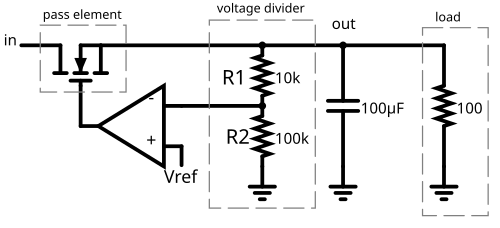
\includegraphics[width=0.6\textwidth]{images/ldo.png}
\caption{LDO circuit. The error amplifier drives the pass element so that the
divided output matches $V_{ref}$; the pass element dissipates
$(V_{in}-V_{out})I_{load}$ as heat.}
\label{fig:ldo}
\end{figure}
%
% buck converter
%
\paragraph{Buck converter (step-down switching regulator):}
\label{fund:buck_converter}
To overcome the thermal inefficiencies of linear regulators, a buck converter is
used.\\\\
A buck converter is a type of switched-mode power supply (SMPS) that
efficiently steps down voltage using a completely different mechanism: instead
of dissipating excess voltage as heat, it rapidly switches the input voltage on
and off.\\\\
%
A standard buck converter circuit consists of a switching transistor, a diode
(or a second transistor for synchronous bucking), an inductor, and a capacitor.\\\\
The transistor chops the input DC voltage into a high-frequency square wave. The
inductor stores energy in a magnetic field during the ``on'' phase and releases
it during the ``off'' phase, while the output capacitor smooths this chopped
energy back into a steady DC voltage.\\\\
%
The efficiency of a buck converter frequently exceeds $90\%$, dramatically
extending battery life in compact, power-constrained designs. However, this
efficiency comes with distinct engineering trade-offs:
\begin{itemize}
    \item \textbf{Complexity and size:} they require external inductors and
    larger capacitors, which consume more physical PCB area.
    \item \textbf{Switching noise:} the high-frequency switching (often between
    \SI{1}{\mega\hertz} and \SI{3}{\mega\hertz}) introduces voltage ripple and
    electromagnetic interference into the system. This noise can severely
    degrade sensitive analog circuits or RF communication modules if the PCB
    layout is not carefully routed.
\end{itemize}
The governing relationship for the ideal continuous-conduction case is
$$V_{out}=D\cdot V_{in},\qquad D=\frac{T_{on}}{T_{total}}$$

\begin{figure}[H]
\centering
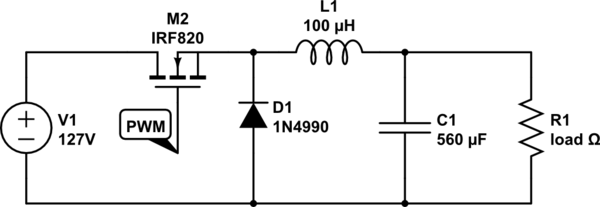
\includegraphics[width=0.6\textwidth]{images/buck.png}
\caption{Buck converter circuit. Energy is transferred to the output through the
inductor rather than dissipated across a pass element, which is what allows
efficiencies above $90\%$.}
\label{fig:buck}
\end{figure}

\subsection{nRF5340}
\label{comp:nrf5340}
The nRF5340 is a wireless ultra-low-power multicore SoC with two fully
programmable Arm Cortex-M33 processors: a network core and an application core.

\subsubsection{Network core}
An Arm Cortex-M33 processor with a reduced feature set designed for
ultra-low-power operation. It is used for radio communication and real-time
processing tasks involving low-level radio protocol layers. Build target:
\begin{verbatim}
    <board_target>/cpunet
\end{verbatim}

\subsubsection{Application core}
A full-featured Arm Cortex-M33 processor that includes DSP instructions and an
FPU. This core is used for tasks that require high performance and for
application-level logic.\\\\
The M33 TrustZone, one of the Cortex-M Security
Extensions (CMSE), can divide the application MCU into a Secure Processing
Environment (SPE) and a Non-Secure Processing Environment (NSPE).\\\\
When the MCU
boots, it always starts executing from the secure area.\\\\
Build targets:
\begin{verbatim}
    <board_target>/cpuapp (TF-M disabled).
    <board_target>/cpuapp/ns (TF-M enabled, SPE firmware alongside the NSPE firmware).
\end{verbatim}
The split-core architecture matters for this project beyond nomenclature: it
means the timing-critical BLE link layer runs on a core that the application
firmware cannot stall.\\\\
A long-running expansion-port transaction on the
application core- for example, a module holding SCL low- therefore cannot
break an active Bluetooth connection.

% ---------------------
\begin{figure}[H]
\centering
\begin{circuitikz}[american, transform shape, scale=0.7, font=\footnotesize]

% nRF5340

    \node[draw, thick, minimum width=4.6cm, minimum height=12cm] (U1) at (0,0){};
    \node[font=\bfseries] at ([yshift=-5mm]U1.north){U1};
    \node[align=center] at (U1.center){nRF5340\\-QKxx};

    % Supply + decoupling bank
    \draw (U1.north) -- ++(0,1.4) coordinate(vdd) node[above, inner sep=1pt]{+1.8V (VDD)};
    \draw (vdd) -- ++(4.8,0) to[C, l={\shortstack{$C14\text{--}C24$\\\SI{100}{\nano\farad}}}] ++(0,-2) node[ground]{};

    % 32 MHz crystal
    \draw ([yshift=55mm]U1.west) coordinate(xc1) -- ++(-1.6,0) coordinate(a1)
        node[midway, above=1pt, font=\scriptsize]{XC1};
    \draw ([yshift=40mm]U1.west) coordinate(xc2) -- ++(-1.6,0) coordinate(a2)
        node[midway, above=1pt, font=\scriptsize]{XC2};
    \draw (a1) -- ++(-1,0.8) coordinate(k1);
    \draw (a2) -- ++(-1,-0.8) coordinate(k2);
    \draw (k1) to[piezoelectric, l=$Y1$, a=\SI{32}{\mega\hertz}] (k2);
    \draw (k1) to[C, l=$C1$, a=\SI{12}{\pico\farad}] ++(-2.6,0) coordinate(r1);
    \draw (k2) to[C, l=$C6$, a=\SI{12}{\pico\farad}] ++(-2.6,0) coordinate(r2);
    \draw (r1) -- (r2);
    \draw ($(r1)!0.5!(r2)$) -- ++(-0.8,0) node[ground]{};

    % 32.768 kHz crystal
    \draw ([yshift=3mm]U1.west) coordinate(xl1) -- ++(-1.6,0) coordinate(d1)
        node[midway, above=1pt, font=\scriptsize]{P0.0/XL1};
    \draw ([yshift=-12mm]U1.west) coordinate(xl2) -- ++(-1.6,0) coordinate(d2)
        node[midway, above=1pt, font=\scriptsize]{P0.1/XL2};
    \draw (d1) -- ++(-1,0.8) coordinate(kk1);
    \draw (d2) -- ++(-1,-0.8) coordinate(kk2);
    \draw (kk1) to[piezoelectric, l=$Y2$, a=\SI{32.768}{\kilo\hertz}] (kk2);
    \draw (kk1) to[C, l=$C13$, a=\SI{12}{\pico\farad}] ++(-2.6,0) coordinate(e1);
    \draw (kk2) to[C, l=$C15$, a=\SI{12}{\pico\farad}] ++(-2.6,0) coordinate(e2);
    \draw (e1) -- (e2);
    \draw ($(e1)!0.5!(e2)$) -- ++(-0.8,0) node[ground]{};

    % DC/DC inductors
    \draw ([yshift=-40mm]U1.west) coordinate(dcc) -- ++(-1.6,0)
        node[midway, above=1pt, font=\scriptsize]{DCC}
        to[L, l=$L4$, a=\SI{10}{\micro\henry}] ++(-3,0) node[ground]{};
    \draw ([yshift=-55mm]U1.west) coordinate(dccd) -- ++(-1.6,0)
        node[midway, above=1pt, font=\scriptsize]{DCCD}
        to[L, l=$L5$, a=\SI{10}{\micro\henry}] ++(-3,0) node[ground]{};

    \draw (U1.south) -- ++(0,-0.9) node[ground]{};

    % RF front end (matching network to antenna)
    \draw ([yshift=16mm]U1.east) coordinate(rf) -- ++(2.4,0) coordinate(m0)
        node[midway, above=1pt, font=\scriptsize]{ANT / RF};
    \draw (m0) to[C, l_={\shortstack[r]{$C8$\\\SI{100}{\pico\farad}}}] ++(0,-2.2) node[ground]{};
    \draw (m0) to[L, l={\shortstack{$L1$\\\SI{15}{\nano\henry}}}] ++(3.2,0) coordinate(m1) node[circ]{}
              to[L, l={\shortstack{$L2$\\\SI{15}{\nano\henry}}}] ++(3.2,0) coordinate(m2) node[circ]{};
    \draw (m1) to[C, l_={\shortstack[r]{$C10$\\\SI{0.7}{\pico\farad}}}] ++(0,-2.2) node[ground]{};
    \draw (m2) to[C, l_={\shortstack[r]{$C9$\\\SI{820}{\pico\farad}}}] ++(0,-2.2) node[ground]{};
    \draw (m2) to[antenna] ++(1.6,0) node[above=4pt, font=\scriptsize]{2.4\,GHz ANT};

    % Digital buses (net-label summary)
    \draw ([yshift=-31mm]U1.east) -- ++(1.2,0) node[right, align=left]
        {\ttfamily QSPI[0:3],SCK,CSN\\ P0.13--P0.18 $\to$ U2};
    \draw ([yshift=-47mm]U1.east) -- ++(1.2,0) node[right, align=left]
        {\ttfamily LCD SPI P0.8--P0.12 $\to$ J2\\ ACC I\textsuperscript{2}C P1.12/P1.13 $\to$ U3\\ PERIPH I\textsuperscript{2}C P0.30/P0.31 $\to$ U6};
\end{circuitikz}
\caption{nRF5340 application SoC (U1). The \SI{32}{\mega\hertz} (Y1) and \SI{32.768}{\kilo\hertz} (Y2) crystals use \SI{12}{\pico\farad} loading capacitors; L4/L5 are the DCC/DCCD DC-DC converter inductors; L1/L2 with C8--C10 form the RF match to the on-board antenna. C14--C24 (\SI{100}{\nano\farad}) are the supply-pin decoupling bank. Digital pins are shown as their KiCad net labels.}
\label{fig:sch_mcu}
\end{figure}

\subsection{Communication protocols}

% big block of UART
\subsubsection{UART}
\textbf{UART}, or \textbf{universal asynchronous receiver-transmitter}, is a
serial communication protocol used widely between integrated circuits due to its
simplicity, configurable data format, and transmission speeds.\\\\
UART works by sending data bits one by one, from the least to the most significant, framed by
start and stop bits, so that precise timing is handled by the communication
channel rather than a shared clock.\\\\
% Amogus
For successful UART communication, the following settings must match on both
sides:
\begin{enumerate}
    \item Voltage level
    \item Baud rate (the rate at which bits are sent)
    \item Parity bit
    \item Data-bit size
    \item Stop-bit size
    \item Flow control
\end{enumerate}
A UART frame consists of five elements:
\begin{itemize}
    \item Idle (logical 1)
    \item Start bit (logical 0)
    \item Data bits: five to nine bits representing the payload
    \item Parity bit: an optional bit after the data bits, used for a parity check
    \item Stop (logical 1): one or two bits representing the stop signal
\end{itemize}
In this project UART is used only as the firmware logging and console channel
during development; no on-board peripheral communicates over it.

\begin{figure}[H]
    \centering
    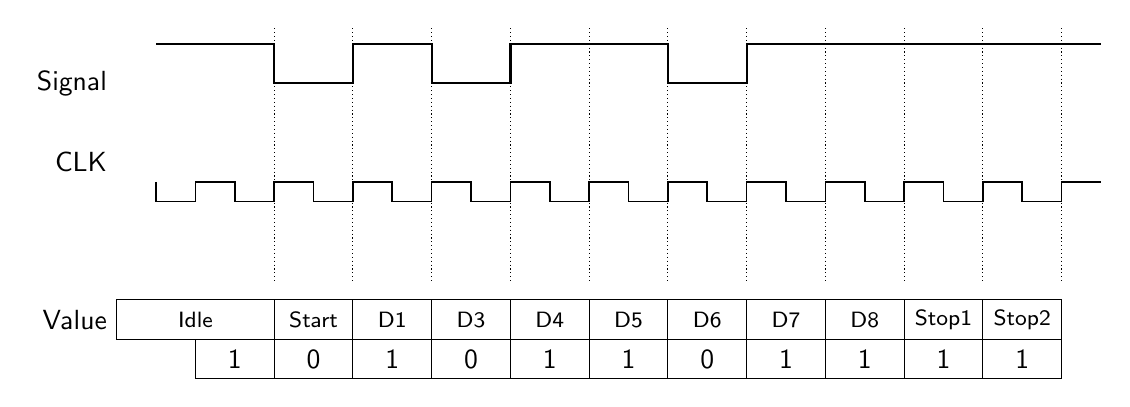
\begin{tikzpicture}[font=\sffamily]

    % 1. Define the Timing Waveforms
    \begin{scope}[shift={(-2,2)}]
        \node[anchor=east] at (-0.5,0) {Signal};
        \draw[thick] (0,0.5) -- (1.5,0.5) % Idle
              -- (1.5,0) -- (2.5,0)     % Start (0)
              -- (2.5,0.5) -- (3.5,0.5) % D1 (1)
              -- (3.5,0) -- (4.5,0)    % D2 (0)
              -- (4.5,0.5) -- (6.5,0.5)% D3, D4 (1, 1)
              -- (6.5,0) -- (7.5,0)   % D5 (0)
              -- (7.5,0.5) -- (12,0.5);% D6, D7, Stop1, Stop2 (1, 1, 1, 1)
    \end{scope}

    % 2. Clock Signal
    \begin{scope}[shift={(-2,0.75)}]
        \node[anchor=east] at (-0.5,0.25) {CLK};
        \draw[semithick] (0,0)
        \foreach \x in {0,1,...,11} {
            -- ++(0,-0.25) -- ++(0.5,0) -- ++(0,0.25) -- ++(0.5,0)
        };
    \end{scope}

    % 3. Vertical Dashed Grid Lines
    \foreach \x in {-0.5,0.5,...,9.5} {
        \draw[densely dotted] (\x, 2.7) -- (\x, -0.5);
    }

    % 4. The Value Table
    \node[anchor=east] at (-2.5,-1) {Value};
    \draw (-2.5,-0.75) rectangle (9.5,-1.25);
    \foreach \x in {-0.5,0.5,...,9.5} {
        \draw (\x,-0.75) -- (\x,-1.75);
    }

    % 5. Row Labels
    \node at (-1, -1.5) {1}; \node at (-1.5, -1) {\footnotesize Idle};
    \node at (0, -1.5) {0}; \node at (0, -1) {\footnotesize Start};
    \node at (1, -1.5) {1}; \node at (1, -1) {\footnotesize D1};
    \node at (2, -1.5) {0}; \node at (2, -1) {\footnotesize D3};
    \node at (3, -1.5) {1}; \node at (3, -1) {\footnotesize D4};
    \node at (4, -1.5) {1}; \node at (4, -1) {\footnotesize D5};
    \node at (5, -1.5) {0}; \node at (5, -1) {\footnotesize D6};
    \node at (6, -1.5) {1}; \node at (6, -1) {\footnotesize D7};
    \node at (7, -1.5) {1}; \node at (7, -1) {\footnotesize D8};
    \node at (8, -1.5) {1}; \node at (8, -1) {\footnotesize Stop1};
    \node at (9, -1.5) {1}; \node at (9, -1) {\footnotesize Stop2};

    % Draw bottom rectangle
    \draw (-1.5,-1.25) rectangle (9.5,-1.75);

    \end{tikzpicture}
    \caption{Example of a UART frame with one start bit, seven data bits, and two stop bits.}
    \label{fig:uart}
\end{figure}

% SPI
\subsubsection{SPI} \label{prot:spi}
SPI (Serial Peripheral Interface) is a synchronous, full-duplex, four-wire
serial communication interface used for short-distance communication between a
controller and multiple target devices.\\\\
Unlike \nameref{prot:i2c}, which is limited by pull-up resistor speeds, SPI is limited only by the maximum clock
frequency of the devices, making it the preferred choice for high-bandwidth
applications like SD cards, LCDs, and high-speed sensors.\\\\
% ;)
SPI uses four dedicated signal lines:
\begin{itemize}
    \item SCLK (serial clock): the clock signal generated by the controller to synchronise data.
    \item MOSI (main out, sub in): the line used to send data from the controller to the target.
    \item MISO (main in, sub out): the line used to send data from the target back to the controller.
    \item CS/SS (chip select / slave select): a dedicated line for each target device. The controller pulls this line low to select the specific device it wants to talk to.
\end{itemize}
In this design SPI carries the display frame data, and its four-bit variant
(QSPI) carries traffic to the external flash.

% i2c
\subsubsection{\texorpdfstring{I\textsuperscript{2}C}{I2C}} \label{prot:i2c}
\nameref{prot:i2c} is a synchronous, multi-controller / multi-target serial communication
bus developed by Philips Semiconductors.\\\\
It is the industry standard for short-distance, intra-board communication between processors and low-speed
peripherals.\\\\
% also check out Minecraft
\nameref{prot:i2c} offers two primary advantages over similar protocols such as
\nameref{prot:spi}:
\begin{itemize}
    \item \textbf{Minimal pin count:} it requires only two signals, regardless of how many devices are on the bus.
    \item \textbf{Software addressing:} unlike \nameref{prot:spi}, which requires a dedicated select line for each peripheral, \nameref{prot:i2c} uses unique 7-bit addresses to communicate with multiple targets on the same bus.
\end{itemize}
The bus consists of two bidirectional lines: the \textbf{serial data (SDA)} and
the \textbf{serial clock (SCL)}.\\\\
Because the devices use open-drain outputs,
both lines must be pulled up to $V_{CC}$ via resistors (typically
$4.7~\text{k}\Omega$ or $10~\text{k}\Omega$).\\\\
% also check out Terraria
These two properties are precisely why \nameref{prot:i2c} was chosen as the expansion
transport in Section~\ref{sec:fwmp}: two contacts serve an unlimited number of
future module types, and addressing is a software matter rather than an
additional physical contact per device.\\\\
Its open-drain nature also has a consequence that Section~\ref{sec:challenges} returns to: a module unplugged
mid-transaction can leave SDA held low and jam the bus for every other
participant.

\begin{figure}[H]
\centering
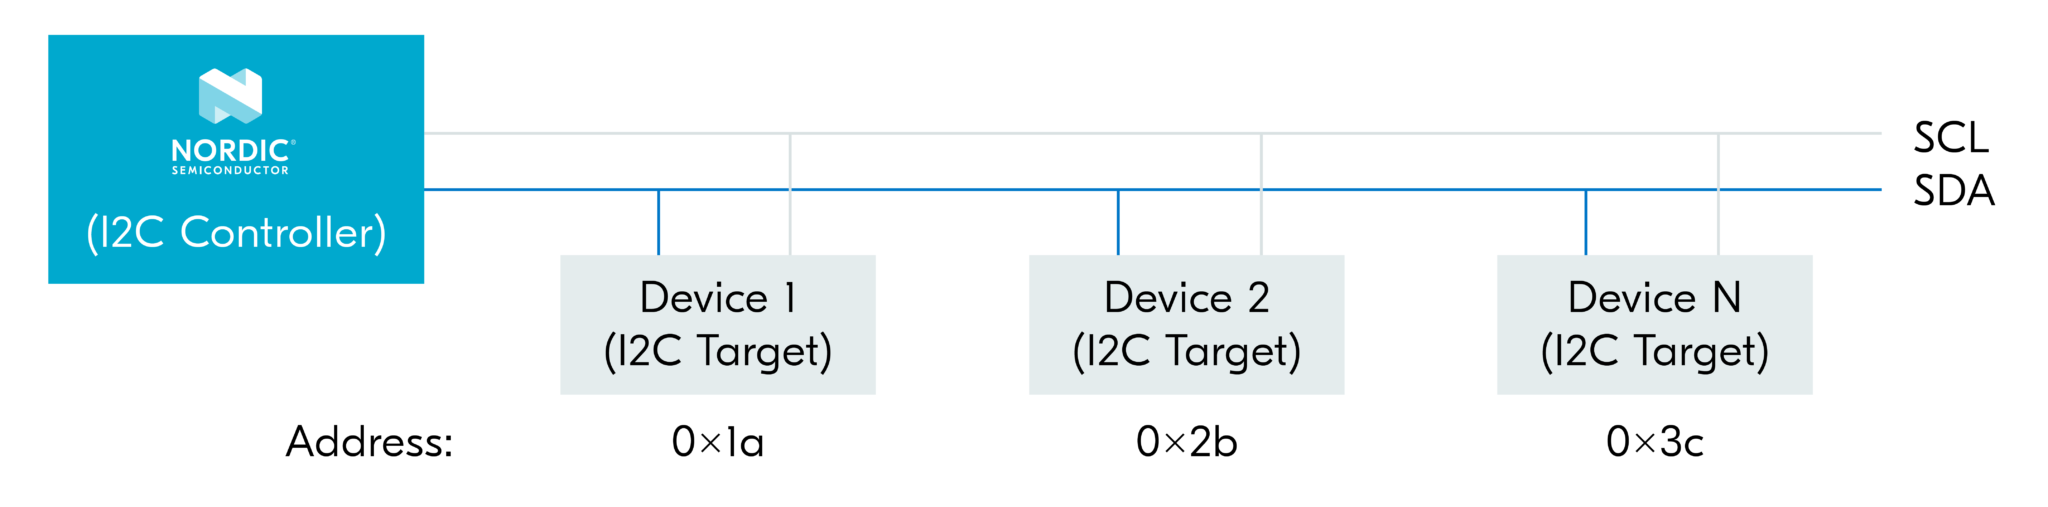
\includegraphics[width=0.6\textwidth]{images/i2c.png}
\caption{\nameref{prot:i2c} bus topology. Open-drain devices pull the lines low; pull-up resistors restore the idle high level, and their value bounds the achievable bus speed.}
\label{fig:i2c}
\end{figure}

% BLE
\subsubsection{BLE}
Bluetooth Low Energy is a wireless personal-area-network technology designed to
provide significantly reduced power consumption compared to ``Classic''
Bluetooth.\\\\
While Classic Bluetooth is intended for continuous data streaming,
BLE is optimised for devices that transmit small amounts of data at infrequent
intervals.\newpage

\textbf{Main characteristics:}
\begin{itemize}
    \item \textbf{Low duty cycle:} BLE devices remain in a sleep state most of the time, waking only for short bursts to advertise their presence or exchange data, which makes the protocol very power efficient.
    \item \textbf{GATT architecture:} data is organised into a Generic Attribute Profile (GATT). This hierarchy consists of services (logical groupings of data) and characteristics (the actual data values, such as a sensor reading), allowing standardised communication across different manufacturers.
    \item \textbf{Connection roles:} the protocol distinguishes between the peripheral (the low-power sensor node) and the central (the powerful device, such as a smartphone, that manages the connection and processes data).
\end{itemize}

The headline efficiency is not automatic, however: it is largely a function of
how the connection interval, slave latency and advertising cadence are chosen,
and those are negotiated at runtime rather than fixed by the specification.
Patel~\cite{patel2025} reports that adaptively managing those parameters, rather
than leaving them at their defaults, is where most of the practical power saving
in Android-paired wearables is found. This is the same argument the present design
makes one layer down, in Section~\ref{sec:fwmp:poll}: the cost of a periodic
activity is set by how often it happens, and that rate should follow demand.

\subsection{Zephyr real-time operating system (RTOS)}
Historically, embedded firmware was written as ``bare-metal'' code, relying on a
single infinite \texttt{while(1)} loop (a superloop) to sequentially poll
sensors, manage timers, and handle communication.\\\\
% soup
While sufficient for simple
microcontrollers, the superloop architecture breaks down in modern IoT and
wearable devices that must concurrently manage a BLE radio stack, graphics
rendering, sensor fusion, and strict power management.\\\\
% sup
To orchestrate this complexity, a \textbf{real-time operating system (RTOS)} is
required. Zephyr is an open-source, highly scalable RTOS hosted by the Linux
Foundation, and serves as the core foundation for advanced vendor toolchains,
particularly for Arm Cortex-M architectures.

\paragraph{Pre-emptive multithreading and scheduling.}
At the heart of Zephyr is its pre-emptive scheduler. Instead of a single loop,
application logic is divided into isolated, independent \textbf{threads}, each
assigned a strict priority level.\\\\
The scheduler guarantees that the
highest-priority thread ready to run always controls the CPU.\\\\
% optimization level: ARK
If a low-priority
thread (for example, updating a display) is executing and a high-priority event
occurs (for example, an incoming BLE packet), the scheduler instantly pre-empts
the low-priority thread, saves its execution state, and hands control to the
high-priority task.\\\\
% turns out BLE is quite convenient
This guarantees deterministic, real-time response latency,
which is critical for maintaining wireless communication links.

\paragraph{Hardware abstraction: Devicetree and Kconfig.}
One of Zephyr's most powerful paradigms is the strict separation of application
logic from hardware description, borrowing heavily from the Linux kernel
architecture:
\begin{itemize}
    \item \textbf{Devicetree (\texttt{.dts}):} a hierarchical data structure that describes the physical PCB hardware. Instead of hardcoding GPIO pins, \nameref{prot:i2c} addresses, or \nameref{prot:spi} frequencies in C code, developers define them in the Devicetree.
    \item \textbf{Kconfig:} a configuration system used to enable or disable specific software features, subsystems, and drivers at compile time, ensuring the final binary footprint remains as small as possible.
\end{itemize}
This architecture makes Zephyr firmware highly portable.\\\\
Transitioning code from
a vendor evaluation board to a custom-designed PCB largely amounts to swapping
the Devicetree overlay, leaving the core application logic untouched, a
property this project depended on directly, since the firmware was developed and
verified on an nRF5340-DK before the custom board existed.

\begin{figure}[H]
\centering
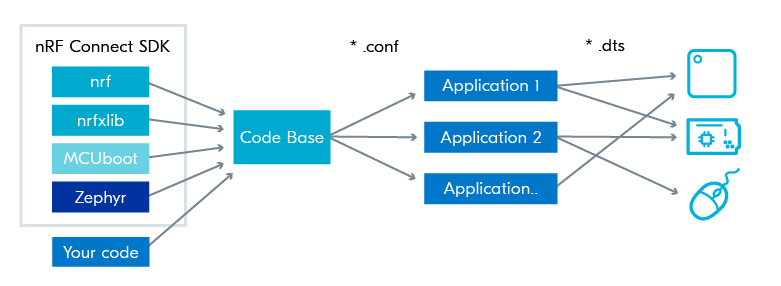
\includegraphics[width=0.6\textwidth]{images/zephyr_build.png}
\caption{Zephyr build process. Devicetree describes the hardware and Kconfig selects the software features; together they produce a board-specific binary from board-independent application code.}
\label{fig:zephyr_build}
\end{figure}

\paragraph{Advanced power management.}
For battery-operated devices, maximising time between charges is the primary
engineering constraint. Zephyr features a natively integrated power-management
(PM) subsystem. It uses a \textbf{tickless kernel}, meaning the OS does not rely
on a constant, battery-draining periodic timer to wake the CPU.\\\\
Instead, when
all threads are idle or waiting for external events, Zephyr calculates the exact
time until the next scheduled task and places the microcontroller into an
ultra-low-power deep-sleep mode.\\\\
Furthermore, device PM allows the OS to
selectively cut power to individual peripheral buses (such as shutting down an
\nameref{prot:i2c} sensor or SPI flash) when they are not actively in use.\\\\

\paragraph{Subsystem integration.}
Zephyr provides production-ready, well-tested subsystems out of the box,
including file systems, USB device stacks, cryptographic libraries, and a fully
qualified open-source BLE host stack. Zephyr's architecture supports split-stack
designs, making it well suited to dual-core SoCs where a dedicated network core
handles the strict timing of the BLE radio while an application core manages the
user interface and sensor data.

\subsection{Inertial measurement and MEMS: the BMI270}
\label{comp:bmi270}
To capture physical kinematics in three-dimensional space, modern embedded
systems use an inertial measurement unit (IMU). The Bosch Sensortec BMI270 is a
highly integrated, ultra-low-power system-in-package featuring a 3D digital
accelerometer and a 3D digital gyroscope in a
$2.5\times3.0\times0.8\,\text{mm}$ LGA-14 package, targeted at wearable and
always-on applications. It is built using
micro-electromechanical systems (MEMS) technology, in which microscopic
mechanical structures are etched directly into the silicon alongside the analog
front-end and digital logic.

Its headline specifications are given in Table~\ref{tab:imu}. Two of them
determine its place in this design: it operates directly from the board's
\SI{1.8}{\volt} digital rail without a dedicated supply, and it speaks
\nameref{prot:i2c} at a 7-bit address selected by the \texttt{SDO} pin, so it shares the
existing sensor bus rather than requiring dedicated pins.

\begin{table}[H]
\centering
\small
\begin{tabular}{@{}l l@{}}
\toprule
\textbf{Parameter} & \textbf{LSM6DSOX} \\
\midrule
Package & LGA-14, $2.5\times3.0\times0.83\,\text{mm}$ \\
Supply (\texttt{VDD}) & \SI{1.71}{\volt} to \SI{3.6}{\volt} \\
I/O supply (\texttt{VDDIO}) & \SI{1.62}{\volt} to \SI{3.6}{\volt} \\
Digital interfaces & \nameref{prot:i2c}, SPI, MIPI I3C \\
\nameref{prot:i2c} address & \texttt{0x6A} / \texttt{0x6B} (selected by \texttt{SA0}) \\
Accelerometer range & $\pm2$ / $\pm4$ / $\pm8$ / $\pm16\,g$ \\
Gyroscope range & $\pm125$ to $\pm2000\,^\circ/\text{s}$ \\
Output data rate & up to \SI{6.66}{\kilo\hertz} \\
FIFO & \SI{9}{\kibi\byte} ``smart'' FIFO with timestamping \\
Embedded processing & Machine Learning Core, Finite State Machine, pedometer \\
Sensor hub & \nameref{prot:i2c} controller for up to 4 external sensors \\
\bottomrule
\end{tabular}
\caption{LSM6DSOX key parameters. The wide \texttt{VDD} range is what allows the part to sit directly on the \SI{1.8}{\volt} digital rail alongside the SoC and the QSPI flash, with no additional regulator.}
\label{tab:imu}
\end{table}

\paragraph{Working principle: accelerometer (linear motion).}
The accelerometer measures linear acceleration using capacitive sensing.
Internally it contains a microscopic mechanical structure consisting of a
tethered ``proof mass'' suspended by silicon springs between fixed electrodes.
When the device experiences acceleration, the inertia of the proof mass causes
it to lag behind the movement of the sensor housing. This displacement changes
the distance ($d$) between the movable mass and the fixed electrodes, altering
the capacitance according to the parallel-plate relation
$$C = \frac{\varepsilon A}{d}$$
The analog front-end measures this minute change in capacitance ($\Delta C$),
converts it to a voltage, and passes it through an analog-to-digital converter
to yield a digital acceleration value on the X, Y, or Z axis.

\paragraph{Working principle: gyroscope (angular velocity).}
The gyroscope measures the rate of rotation by exploiting the \textbf{Coriolis
effect}. Inside the MEMS structure a proof mass is continuously driven to
vibrate at a high resonant frequency in a specific plane. When the sensor
rotates about an axis, the vibrating mass experiences the Coriolis force, which
acts perpendicular to both the direction of vibration and the axis of rotation.
The Coriolis force is proportional to the angular velocity $\vec{\Omega}$:
$$\vec{F}_c = -2m (\vec{\Omega} \times \vec{v})$$
where $m$ is the mass and $\vec{v}$ its instantaneous velocity. This force
displaces the mass into a secondary sensing plane, which is again measured
capacitively and digitised.

\paragraph{Advanced architecture: embedded processing and smart interrupts.}
While many IMUs simply output raw X, Y, and Z data over \nameref{prot:i2c} or SPI,
continuous polling of that data forces the main microcontroller
(\nameref{comp:nrf5340}) to remain awake, drawing significant battery power. The
defining advantage of the LSM6DSOX is that it can do a substantial amount of
that work itself, in three layers of increasing sophistication:

\begin{itemize}
  \item \textbf{Fixed-function embedded features.} A hardware pedometer (step
  detector and step counter), tilt detection, significant-motion detection,
  free-fall, wake-up, and 6D/4D orientation are implemented in the sensor and
  require only register configuration. Each can be routed to one of the two
  interrupt pins, so the host is notified of an \emph{event} rather than being
  handed a stream of samples to interpret.

  \item \textbf{Finite State Machine (FSM).} A set of programmable state
  machines that trigger on user-defined sequences of sensor conditions, for
  gesture recognition beyond the fixed-function set.

  \item \textbf{Machine Learning Core (MLC).} An in-sensor decision-tree
  classifier. Trees are trained offline on labelled motion data using ST's MEMS
  Studio tooling and loaded as a configuration (\texttt{.ucf}) file at
  initialisation; the sensor then performs continuous activity classification:
  walking, running, stationary, and raises an interrupt when the
  classified class changes.
\end{itemize}

The intended consequence for a wearable is that the IMU performs continuous,
real-time context and gesture recognition at a small fraction of a milliampere,
allowing the main MCU to remain in deep sleep until the sensor announces that a
specific physical event has occurred. The \SI{9}{\kibi\byte} FIFO reinforces
this: even where the host must see raw samples, it can sleep while the sensor
buffers them and wake once per batch rather than once per sample.

The firmware exploits the first of these three layers: the wake-up (activity)
detector is configured to assert INT1 on motion, and the application core
blocks until it fires rather than polling. Step counting itself still runs on
the host, inside a bounded active window opened by that interrupt; The
design is described in Section~\ref{sec:impl}, and moving it into the sensor's
own pedometer is discussed in Section~\ref{sec:future}.

\subsection{Power management IC: the nPM1300}
\label{comp:npm1300}
In ultra-low-power wearable and IoT designs, efficient power conversion and
rigorous battery management are critical for maximising battery longevity while
maintaining a compact form factor. The alternative research direction is to
attack the supply rather than the load --- integrating harvesting, conversion and
storage into a single self-chargeable module~\cite{maharjan2020} --- but that
trades a well-understood recharge cycle for a dependence on ambient conditions,
which is not a trade a watch that must work on demand can currently make. This
design therefore keeps a conventional Li-Po cell and concentrates on conversion
efficiency and on cutting idle draw.\\\\
The Nordic Semiconductor nPM1300 is a
dedicated, highly integrated power management integrated circuit (PMIC) designed
to complement low-power microcontrollers such as the \nameref{comp:nrf5340}.\\
Rather than relying on scattered discrete regulators, battery chargers, and
supervisor ICs, the nPM1300 consolidates the essential power-management building
blocks into a single $5\times 5\,\text{mm}$ QFN32 package.\\\\
It incorporates dual
high-efficiency synchronous buck converters, two linear regulators / load
switches, a full-featured linear Li-ion/Li-Po battery charger with automatic
power-path management, an on-chip Coulomb counter for fuel gauging, and system
supervisor logic.

\paragraph{Dual synchronous buck converters.}
Building on the switched-mode principles introduced in
\nameref{fund:buck_converter}, the nPM1300 integrates two step-down switching
regulators.\\\\
Unlike discrete buck implementations that require external power
MOSFETs and control feedback loops, the nPM1300 embeds the switching transistors
and the PWM/PFM control circuitry internally.\\\\
Each converter requires only a
miniature external inductor ($L = \SI{2.2}{\micro\henry}$) and filtering
capacitor ($C = \SI{10}{\micro\farad}$) to achieve conversion efficiencies
exceeding $90\%$ (Figure~\ref{fig:sch_power}):
\begin{itemize}
    \item \textbf{BUCK1 (\SI{1.8}{\volt} rail):} configured by external resistor $R_8 = \SI{47}{\kilo\ohm}$ on the \texttt{VSET1} pin. This rail powers the main digital logic, flash memory, and sensor interfaces, including the \nameref{comp:nrf5340} core supply alongside the \nameref{fund:decoupling_capacitors}-filtered peripheral rails.
    \item \textbf{BUCK2 (\SI{3.3}{\volt} rail):} configured by external resistor $R_9 = \SI{250}{\kilo\ohm}$ on the \texttt{VSET2} pin. 
    This rail provides the higher operating voltage required by external peripherals, such as the display backlight, the off-board I/O headers, and, critically for this project, the expansion port (Figures~\ref{fig:sch_periph} and \ref{fig:sch_io}).
\end{itemize}
During ultra-low-power sleep states the regulators automatically switch from PWM
to PFM mode, reducing quiescent current to microampere levels.

\paragraph{Battery charging and power-path management.}
The nPM1300 incorporates an autonomous linear battery charger supporting
single-cell lithium-ion and lithium-polymer chemistries connected via the
battery terminal ($J4$):
\begin{itemize}
    \item \textbf{CC/CV charging profile:} the charger operates in constant-current / constant-voltage mode, with programmable termination voltages (\SI{3.5}{\volt} to \SI{4.45}{\volt}), configurable charge currents up to \SI{800}{\milli\ampere}, and automatic trickle charging for deeply depleted cells.
    \item \textbf{Dynamic power path:} the PMIC monitors the $V_{\text{BUS}}$ input from the USB pogo-pin interface (Figure~\ref{fig:sch_io}). When $V_{\text{BUS}}$ (\SI{5}{\volt}) is present, power-path management routes power directly from the external source to the system buck regulators while directing the remaining current to charge the battery. When USB power is detached, the system transitions to battery operation with no supply glitch, preventing unexpected brownout resets on the \nameref{comp:nrf5340}.
    \item \textbf{Thermal safety (JEITA):} by interfacing with an external NTC thermistor, the charger continuously adjusts current limits and target voltages based on battery temperature, enforcing standard JEITA safety boundaries to prevent thermal runaway.
\end{itemize}

\paragraph{Fuel gauging and Coulomb counter.}
Accurate state-of-charge (SoC) estimation is notoriously difficult in
lithium-based batteries because the open-circuit discharge voltage remains
virtually flat throughout most of the discharge cycle.\\\\
Relying solely on voltage
measurements leads to severe inaccuracies under dynamic load transitions. To
overcome this limitation, the nPM1300 integrates an autonomous hardware
\textbf{Coulomb counter}, which continuously samples the bidirectional current
across an internal sense element and integrates the total charge over time:
$$Q(t) = Q_0 + \int_{0}^{t} I_{\text{batt}}(\tau)\, d\tau$$
Coupled with high-accuracy internal ADCs monitoring instantaneous battery
voltage, load current, and die temperature, the fuel gauge provides reliable
real-time capacity metrics to the host without requiring continuous,
power-draining CPU sampling routines.

\paragraph{Host control, system supervisor, and Zephyr integration.}
The nPM1300 operates in close conjunction with the host processor:
\begin{itemize}
    \item \textbf{Two-wire digital interface:} all internal registers, regulator set-points, charger telemetry, and interrupt masks are accessed by the \nameref{comp:nrf5340} over the standard \nameref{prot:i2c} bus.
    \item \textbf{System supervisor and hard reset:} the IC integrates hardware watchdog monitoring, power-loss reset circuitry, and configurable GPIO/button controller logic capable of detecting wake-up events and long-press power-cycle commands from physical push-buttons (SW2/SW3 in Figure~\ref{fig:sch_io}).
    \item \textbf{Zephyr driver architecture:} in firmware the nPM1300 is integrated into the Zephyr ecosystem via native multi-function device (MFD), regulator, and charger drivers (\texttt{CONFIG\_REGULATOR\_NPM1300}, \texttt{CONFIG\_CHARGER\_NPM1300}). The hardware layout is defined in the Devicetree, allowing Zephyr's power-management subsystem to throttle or disable voltage rails, handle charger interrupts, and transition the system into low-power sleep states when idle.
\end{itemize}

% ---------------------
\begin{figure}[H]
\centering
\begin{circuitikz}[american, transform shape, scale=0.9, font=\footnotesize]

% PMIC
    \node[draw, thick, minimum width=3.4cm, minimum height=5.4cm] (U4) at (0,0){};
    \node[font=\bfseries] at ([yshift=-5mm]U4.north){U4};
    \node[align=center] at (U4.center){nPM1300\\-QEXX};
    \node[font=\scriptsize] at ([yshift=4mm]U4.south){PMIC};

    % Inputs
    \draw ([yshift=-9mm]U4.north west) -- ++(-1.7,0) node[above left]{+BATT (J4)};
    \draw ([yshift=-17mm]U4.north west) -- ++(-1.7,0) node[above left]{VBUS (J3)};

    % Set-point resistors
    \draw ([yshift=15mm]U4.south west) coordinate(vs1) node[above left, inner sep=1pt]{VSET1}
        -- ++(-3,0) to[R, l=\SI{47}{\kilo\ohm}, a=$R8$] ++(0,-2.1) node[ground]{};
    \draw ([yshift=5mm]U4.south west) coordinate(vs2) node[above left, inner sep=1pt]{VSET2}
        -- ++(-1.3,0) to[R, l=\SI{250}{\kilo\ohm}, a=$R9$] ++(0,-2.1) node[ground]{};

    \draw (U4.south) -- ++(0,-0.6) node[ground]{};

    % BUCK1 -> +1.8 V
    \draw ([yshift=-10mm]U4.north east) coordinate(sw1) node[above right, inner sep=1pt]{SW1}
        -- ++(0.5,0) to[L, l=\SI{2.2}{\micro\henry}, a=$L7$] ++(3,0)
        coordinate(o1) node[circ]{} -- ++(1,0) node[above right, font=\bfseries]{+1.8V};
    \draw (o1) to[C, l_=\SI{10}{\micro\farad}, a^=$C29$] ++(0,-2) node[ground]{};

    % BUCK2 -> +3.3 V
    \draw ([yshift=-45mm]U4.north east) coordinate(sw2) node[above right, inner sep=1pt]{SW2}
        -- ++(0.5,0) to[L, l=\SI{2.2}{\micro\henry}, a=$L6$] ++(3,0)
        coordinate(o2) node[circ]{} -- ++(1,0) node[above right, font=\bfseries]{+3.3V};
    \draw (o2) to[C, l_=\SI{10}{\micro\farad}, a^=$C30$] ++(0,-2) node[ground]{};
\end{circuitikz}
\caption{Power tree. A single-cell Li-Po (J4) and the USB \texttt{VBUS} rail (J3) feed the nPM1300 PMIC (U4). BUCK1 (L7 + C29) generates the \SI{1.8}{\volt} core/IO rail; BUCK2 (L6 + C30) generates the \SI{3.3}{\volt} peripheral rail. R8 and R9 program the two buck output voltages.}
\label{fig:sch_power}
\end{figure}

%\newpage
% =================================================================
\section{System design overview}
\label{sec:design}

This section describes what the system does and how the different functional blocks connect to each other. The lower-level implementation details are covered later in Section~\ref{sec:impl}.

\subsection{Requirements}

We derived our hardware and software requirements directly from the main project objective:

\begin{table}[H]
\centering
\small
\begin{tabular}{@{}p{1.4cm} p{5.6cm} p{7cm}@{}}
\toprule
\textbf{ID} & \textbf{Requirement} & \textbf{Rationale / acceptance} \\
\midrule
R1 & Wrist-wearable form factor & Board must fit a plausible watch case; Board radius: 22.9856 mm \\\\
R2 & Single-cell Li-Po operation with USB charging & Charging and power path handled on-board, no external charger \\\\
R3 & Days of battery life at typical duty cycle & Switching conversion throughout; MCU idle in deep sleep \\\\
R4 & BLE connectivity to a phone & Standard GATT services; battery level notified to central \\\\
R5 & Motion sensing with step counting, without continuous host polling & Met for the idle case: the sensor's wake-up detector raises an interrupt and the host sleeps until then. Step detection itself remains host-side but runs only while the wrist is moving (Section~\ref{sec:impl}) \\\\
R6 & Colour display with touch input & SPI display + capacitive touch controller \\\\
R7 & Non-volatile storage for settings and logs & External QSPI flash with a file system \\\\
R8 & \textbf{Documented expansion port} & Four contacts, $\le$ 2 signal lines, \SI{3.3}{\volt} module supply \\\\
R9 & \textbf{Runtime discovery of unknown modules} & Host firmware must not need prior knowledge of a module \\\\
R10 & \textbf{Robustness against a faulty or hostile module} & No module-supplied value may be used before validation; a jammed bus must be recoverable \\\\
R11 & Firmware portable between the DK and the custom board & Devicetree overlay only; no application-code changes \\\\
\bottomrule
\end{tabular}
\caption{System requirements. R8--R10 are specific to this project's contribution and are addressed in Section~\ref{sec:fwmp}.}
\label{tab:requirements}
\end{table}

\newpage

\subsection{System architecture}

As shown in our block diagram (Figure~\ref{fig:block}), power comes from either the battery or the USB pogo header and goes into the PMIC. The PMIC converts this into two main rails: a \SI{1.8}{\volt} digital rail and a \SI{3.3}{\volt} peripheral rail. All the on-board digital logic runs at \SI{1.8}{\volt}. Everything that crosses the enclosure boundary runs at \SI{3.3}{\volt}. We used a bidirectional level shifter to connect the \SI{1.8}{\volt} \nameref{prot:i2c} bus from the SoC to the \SI{3.3}{\volt} expansion port, which is what makes the expansion port usable by ordinary \SI{3.3}{\volt} hardware.

% System architecture diagram
\begin{figure}[H]
\centering
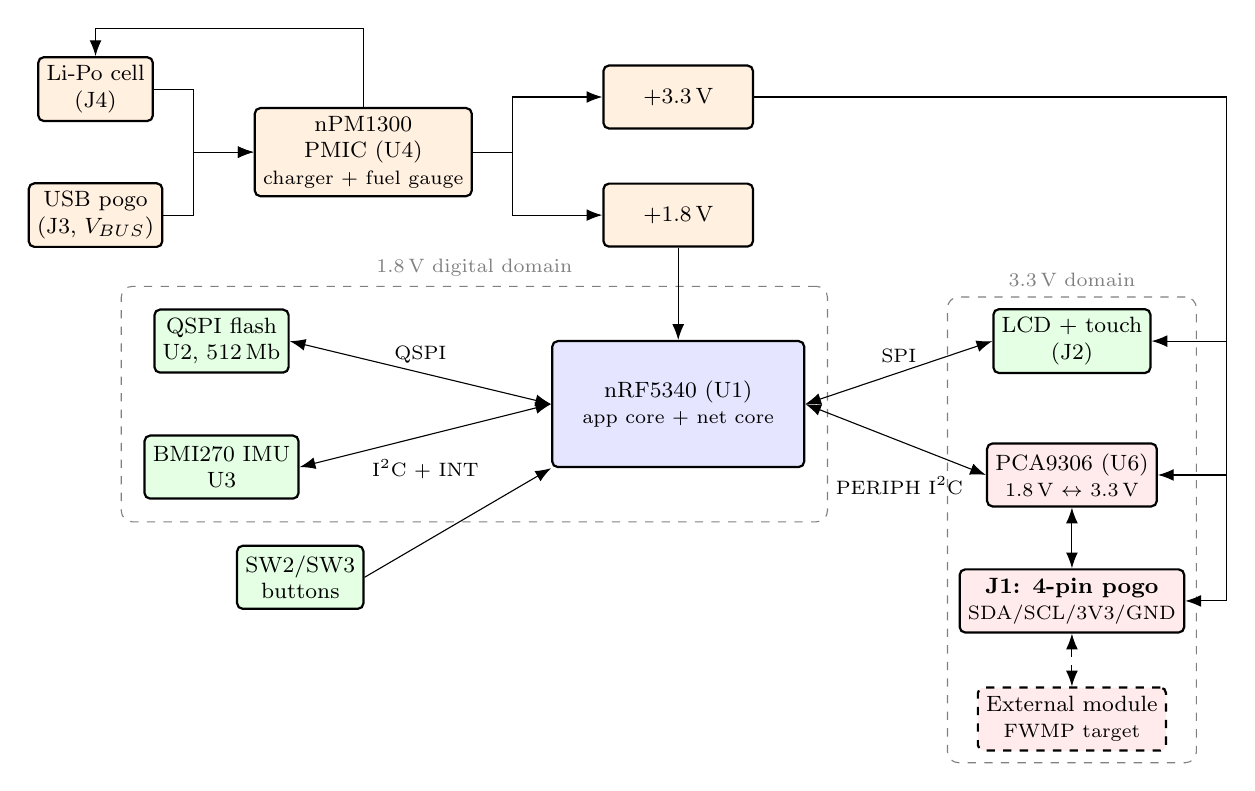
\begin{tikzpicture}[
  font=\footnotesize,
  blk/.style={draw, thick, rounded corners=2pt, minimum height=8mm, align=center, inner sep=3pt},
  pwr/.style={blk, fill=orange!12},
  soc/.style={blk, fill=blue!10},
  per/.style={blk, fill=green!10},
  ext/.style={blk, fill=red!8},
  >={Latex[length=2mm]}
]

% Power column
\node[pwr] (batt) at (-1,0) {Li-Po cell\\(J4)};
\node[pwr] (usb)  at (-1,-1.6) {USB pogo\\ (J3, $V_{BUS}$)};
\node[pwr] (pmic) at (2.4,-0.8) {nPM1300\\PMIC (U4)\\{\scriptsize charger + fuel gauge}};

\draw[->] (batt.east) -- ++(0.5,0) |- (pmic.west);
\draw[->] (usb.east)  -- ++(0.38,0) |- (pmic.west);

% Rails
\node[pwr, minimum width=1.9cm] (r18) at (6.4,-0.1) {+3.3\,V};
\node[pwr, minimum width=1.9cm] (r33) at (6.4,-1.6) {+1.8\,V};
\draw[->] (pmic.east) -- ++(0.5,0) |- (r18.west);
\draw[->] (pmic.east) -- ++(0.5,0) |- (r33.west);
% also use the pmic for charging
\draw[->] (pmic.north) -- ++(0, 1) -| (batt.north);

% SoC
% 1.8V -> SoC
\node[soc, minimum width=3.2cm, minimum height=1.6cm] (soc) at (6.4,-4.0)
  {nRF5340 (U1)\\{\scriptsize app core + net core}};
\draw[->] (r33.south) -- (soc.north);

% Peripherals (1.8 V side)
\node[per] (flash) at (0.6,-3.2) {QSPI flash\\U2, 512\,Mb};
\node[per] (imu)   at (0.6,-4.8) {BMI270 IMU\\U3};
\draw[<->] (soc.west) -- node[above, font=\scriptsize]{QSPI} (flash.east);
\draw[<->] (soc.west) -- node[below, yshift=-5pt, font=\scriptsize]{I\textsuperscript{2}C + INT} (imu.east);

% Peripherals (3.3 V side)
\node[per] (lcd) at (11.4,-3.2) {LCD + touch\\(J2)};
\node[ext] (ls)  at (11.4,-4.9) {PCA9306 (U6)\\{\scriptsize 1.8\,V $\leftrightarrow$ 3.3\,V}};
\node[ext] (pogo) at (11.4,-6.5) {\textbf{J1: 4-pin pogo}\\{\scriptsize SDA/SCL/3V3/GND}};
\node[ext, dashed] (mod) at (11.4,-8.0) {External module\\{\scriptsize FWMP target}};

\draw[<->] (soc.east) -- node[above, font=\scriptsize]{SPI} (lcd.west);
\draw[<->] (soc.east) -- node[below, font=\scriptsize, yshift=-10pt]{\ PERIPH I\textsuperscript{2}C} (ls.west);
\draw[<->] (ls) -- (pogo);
\draw[<->, dashed] (pogo) -- (mod);
% 3.3V -> peripherals
% connect the 3.3V rail to the 3.3V domain
\draw[->] (r18.east) -- ++(6,0) |- (lcd.east);
\draw[->] (r18.east) -- ++(6,0) |- (ls.east);
\draw[->] (r18.east) -- ++(6,0) |- (pogo.east);
% Buttons
\node[per] (btn) at (1.6,-6.2) {SW2/SW3\\buttons};
\draw[<-] (soc.south west) -- (btn.east);

% Dashed domain separators
\begin{scope}[on background layer]
  \node[draw, dashed, gray, rounded corners, fit=(flash)(imu)(soc), inner sep=8pt,
        label={[gray, font=\scriptsize]above:1.8\,V digital domain}] {};
  \node[draw, dashed, gray, rounded corners, fit=(lcd)(pogo)(mod), inner sep=4pt,
        label={[gray, font=\scriptsize]above:3.3\,V domain}] {};
\end{scope}

\end{tikzpicture}
\caption{FinWatch system architecture. Power (orange) enters from the battery or the USB pogo header and is converted by the PMIC into the \SI{1.8}{\volt} digital rail and the \SI{3.3}{\volt} peripheral rail. On-board peripherals (green) attach directly to the SoC; everything crossing the enclosure boundary (red) does so at \SI{3.3}{\volt} through the level shifter, including the expansion port J1 and any attached module.}
\label{fig:block}
\end{figure}

\newpage

\subsection{Component selection}
We selected every major part by comparing it against alternatives, and we summarized our reasoning in Table~\ref{tab:selection}. However, it's worth noting that two of these choices were eventually forced by component availability rather than pure technical merit, which we discuss later in Section~\ref{sec:challenges}.

\begin{table}[H]
\centering
\small
\begin{tabular}{@{}p{2.4cm} p{3.3cm} p{3.2cm} p{5cm}@{}}
\toprule
\textbf{Function} & \textbf{Chosen part} & \textbf{Alternatives} & \textbf{Reason for choice} \\
\midrule
SoC & nRF5340-QKxx, bare IC (U1) & nRF52840, ESP32-C3, STM32WB; or the same SoC as a pre-certified module (e.g.\ u-blox NORA-B10) & Dual core isolates the BLE stack from application timing; best-in-class sleep current; first-class Zephyr support. The bare IC rather than a module: smaller, cheaper, and it places the RF front end and fine-pitch escape inside the project's scope --- at the cost of owning the RF design and any certification (Section~\ref{sec:discussion}) \\
PMIC & nPM1300 (U4) & Discrete buck + MCP73831 charger + supervisor & One package replaces four; integrated fuel gauge; native Zephyr drivers; same vendor as the SoC \\
IMU & BMI270 (U3) & LSM6DSOX (original choice), ICM-42688 & Operates from the \SI{1.8}{\volt} rail; on-sensor pedometer, FSM, and Machine Learning Core can keep the MCU asleep; available when the LSM6DSOX was not (Section~\ref{sec:challenges}) \\
Flash & MX25U51245G (U2) & Internal 1\,MB only; smaller SPI NOR & \SI{512}{\mega\bit} at \SI{1.8}{\volt}, QSPI-capable, enough for fonts, assets, and logs \\
Level shifter & PCA9306 (U6) & Discrete MOSFET shifters; TXS0102 & Purpose-built for \nameref{prot:i2c}; passes open-drain semantics correctly in both directions \\
Display & Waveshare LCD + capacitive touch (J2) & Bare panel + separate controller & Single FPC connector, known-good driver, reduces mechanical risk \\
Expansion & 4-pin pogo (J1) & Board-to-board connector; USB-C alt mode & Sealed-surface contacts, no cavity through the case, cheap to implement on the module side \\
\bottomrule
\end{tabular}
\caption{Component selection and the alternatives considered.}
\label{tab:selection}
\end{table}

\subsection{Firmware architecture}

We organized the firmware into nine subsystems. Each subsystem handles a specific piece of hardware and exposes a minimal C interface, along with a set of Zephyr threads running at fixed priorities. Table~\ref{tab:threads} lists the threads we used; keep in mind that lower numbers mean higher priority.

\begin{table}[H]
\centering
\small
\begin{tabular}{@{}l c r p{7.2cm}@{}}
\toprule
\textbf{Thread} & \textbf{Priority} & \textbf{Stack} & \textbf{Responsibility} \\
\midrule
Display / LVGL & 7 & - & Renders the UI and services the touch input device \\
Sensor & 8 & 2048\,B & Blocks on the BMI270 INT1 wake-up interrupt; samples at \SI{10}{\hertz} only inside an active window, detects steps, fires the motion callback \\
Update & 9 & 1024\,B & 1\,Hz watch-face refresh: time, steps; battery every 10\,s \\
Expansion & 10 & 1536\,B & Presence polling, enumeration, input/output reports \\
\bottomrule
\end{tabular}
\caption{Firmware thread model. The expansion port is deliberately the lowest-priority thread on the system: a module must never be able to delay the display, the sensor, or the watch face by holding the bus.}
\label{tab:threads}
\end{table}
The way we ordered these priorities was a deliberate design choice based on system safety. We set the expansion thread to run at the absolute lowest priority in the system. This means that if an attached module responds slowly or holds the clock line indefinitely, it only ruins its own responsiveness. Since the BLE stack also runs on a separate physical core, no misbehaviour of an external module on the bus can freeze the user interface or drop the radio link. We also made the startup process fault-tolerant: inside \texttt{main()}, if any subsystem except the display fails to initialize, we log a warning and let the boot process continue. The expansion port is fundamentally optional hardware, so it must never prevent the watch from booting.

\subsection{Use cases}

\paragraph{Use case 1: everyday wear.} When no module is attached, the main MCU sleeps. The IMU watches for motion on its own. When the user raises their wrist, the sensor asserts an interrupt, the display wakes up, and the sensor thread samples at \SI{10}{\hertz} to count steps. A background thread updates the time and step count every second, and checks the battery every \SI{10}{\second}. The expansion thread just probes the \nameref{prot:i2c} bus once a second and finds nothing.

\paragraph{Use case 2: attaching a module.} When the user clips a module onto the pogo contacts, the watch detects it after two consecutive successful probes. The host reads the module's descriptor, validates it, and finds out its name, its report sizes, and how often it wants to be polled. A new screen appears in the UI to show the module's data. If the user switches to a different screen, the polling rate backs off from \SI{50}{\milli\second} to \SI{250}{\milli\second} to save battery. If the module is pulled off, three consecutive failed probes trigger the teardown process. None of this requires the watch firmware to know anything about the specific module beforehand.

\newpage
% =================================================================
\section{The FinWatch Module Protocol (FWMP)}
\label{sec:fwmp}

This section breaks down our main contribution to the project: the protocol that lets any third-party hardware become a working part of a sealed smartwatch.\\
The protocol is built on three layers -- electrical, logical, and behavioral.\\
Our guiding design principle across all three layers was simple: the watch must be able to accept a completely unknown module from an untrusted source, without needing any prior firmware updates, and without any fault in that module's data or bus behavior being able to crash the watch.

\subsection{The electrical contract}

For the expansion port, we went with connector J1, which is a four-contact pogo-pin interface located on the outside of the watch case. Table~\ref{tab:j1} details the electrical layout of these pins.

\begin{table}[H]
\centering
\small
\begin{tabular}{@{}c l l p{7.4cm}@{}}
\toprule
\textbf{Pin} & \textbf{Signal} & \textbf{Direction} & \textbf{Notes} \\
\midrule
1 & \texttt{+3V3} & Watch $\to$ module & From PMIC BUCK2. Module current is bounded by the platform budget; exceeding it is a specification violation \\
2 & \texttt{SDA} & Bidirectional & Open drain, \SI{3.3}{\volt} logic. \\
3 & \texttt{SCL} & Watch $\to$ module & Open drain, \SI{3.3}{\volt} logic, watch is always the bus controller. \\
4 & \texttt{GND} & - & \\
\bottomrule
\end{tabular}
\caption{FWMP electrical interface (connector J1).}
\label{tab:j1}
\end{table}

Choosing exactly four contacts had three major consequences that shaped the rest of our design:

\begin{itemize}
  \item \textbf{Pull-ups belong to the watch.} We placed the \nameref{prot:i2c} pull-up resistors (R2/R3 on the \SI{1.8}{\volt} side) inside the watch.\\
  A compliant external module must add its own pull-ups, the decition to not add pull ups on the watch side was intentional, because many boards that can be used to implement a module will have their own pull-up requirements(Raspberry Pi, Arduino).

  \item \textbf{There is no interrupt line.} Adding a fifth contact would have given us event-driven notifications, but we decided against it to save enclosure space and avoid mechanical alignment issues. Instead, we trade power for contacts: the watch discovers module presence and data availability strictly by polling.

  \item \textbf{The domain crossing is mandatory.} The nRF5340's I/O pins run at \SI{1.8}{\volt}, but almost all hobbyist sensors need \SI{3.3}{\volt}. We added a PCA9306 level shifter between the SoC and the J1 connector. This costs us one extra component and a pair of pull-ups, but it makes the requirement that the port can talk to standard \SI{3.3}{\volt} \nameref{prot:i2c} hardware actually work.
\end{itemize}

\subsection{The logical contract: register map}

We set the module to act as an \nameref{prot:i2c} target at a fixed 7-bit address of \texttt{0x42}.\\
We chose this specific address because it sits safely outside the reserved \nameref{prot:i2c} ranges (\texttt{0x00}--\texttt{0x07} and \texttt{0x78}--\texttt{0x7F}). \\
Since this \nameref{prot:i2c} bus is dedicated entirely to the expansion port and only connects to one module at a time, a fixed address is all we need. \\
This avoids the added complexity of implementing dynamic address assignment on a bus that doesn't have out-of-band signaling. \\
The module exposes a flat register space, which we read using the standard EEPROM method: write the offset, send a repeated START, and read the bytes. \\
As shown in the mapping below, the lower registers store the static descriptor, while the higher registers handle the runtime input and output reports.

\begin{table}[H]
\centering
\small
\begin{tabular}{@{}l l l p{6.6cm}@{}}
\toprule
\textbf{Offset} & \textbf{Name} & \textbf{Size} & \textbf{Meaning} \\
\midrule
\multicolumn{4}{@{}l}{\textit{Descriptor header (fixed, 10 bytes)}}\\
\texttt{0x00} & \texttt{MAGIC0}    & 1 & \texttt{0x46} (`F') \\
\texttt{0x01} & \texttt{MAGIC1}    & 1 & \texttt{0x57} (`W') \\
\texttt{0x02} & \texttt{PROTO\_VER}& 1 & Protocol version; \texttt{0x01} for FWMP v1 \\
\texttt{0x03} & \texttt{DESC\_LEN} & 1 & Total descriptor length: header + TLVs + CRC \\
\texttt{0x04} & \texttt{VID}       & 2 & Vendor ID, little-endian \\
\texttt{0x06} & \texttt{PID}       & 2 & Product ID, little-endian \\
\texttt{0x08} & \texttt{CAPS}      & 1 & Capability bitmask (Table~\ref{tab:caps}) \\
\texttt{0x09} & \texttt{N\_TLV}    & 1 & Number of TLV entries that follow \\
\texttt{0x0A} & TLV area           & var & TLV entries, then a trailing CRC-16 \\
\midrule
\multicolumn{4}{@{}l}{\textit{Runtime registers}}\\
\texttt{0x80} & \texttt{STATUS}    & 1 & Status bits (Table~\ref{tab:caps}) \\
\texttt{0x81} & \texttt{SEQ}       & 1 & Incremented by the module on each new input report \\
\texttt{0x82} & \texttt{INPUT}     & var & Input report, length declared in the descriptor \\
\texttt{0xC0} & \texttt{OUTPUT}    & var & Output report written by the host \\
\bottomrule
\end{tabular}
\caption{FWMP v1 register map. \texttt{STATUS} and \texttt{SEQ} are adjacent by design so that a single two-byte read answers both ``is there new data?'' and ``is it data I have already seen?''.}
\label{tab:regmap}
\end{table}

\begin{table}[H]
\centering
\small
\begin{tabular}{@{}l l l@{}}
\toprule
\textbf{Field} & \textbf{Bit} & \textbf{Meaning} \\
\midrule
\texttt{CAPS} & 0 (\texttt{CAP\_INPUT})  & Module produces input reports \\
\texttt{CAPS} & 1 (\texttt{CAP\_OUTPUT}) & Module accepts output reports \\
\texttt{STATUS} & 0 (\texttt{DATA\_READY}) & An unread input report is waiting \\
\texttt{STATUS} & 1 (\texttt{ERROR})       & Module-side error condition \\
\texttt{STATUS} & 2 (\texttt{BUSY})        & Module cannot service a transaction now \\
\bottomrule
\end{tabular}
\caption{Capability and status bit definitions.}
\label{tab:caps}
\end{table}

\subsection{The descriptor: self-description through TLVs}

The fixed header tells the host that a module is connected and which protocol version it uses, but it doesn't tell us what the module actually is. \\
To solve this, we used a sequence of Type-Length-Value (TLV) entries located between the header and the trailing CRC. \\
Each TLV entry consists of one type byte, one length byte, and the actual payload bytes.

\begin{table}[H]
\centering
\small
\begin{tabular}{@{}l l l p{7cm}@{}}
\toprule
\textbf{Type} & \textbf{Name} & \textbf{Payload} & \textbf{Meaning} \\
\midrule
\texttt{0x01} & \texttt{NAME} & ASCII, $\le$ 24 B & Human-readable module name, not NUL-terminated on the wire \\
\texttt{0x02} & \texttt{INPUT\_REPORT} & 3 B & \texttt{[len][poll\_hint\_ms:2 LE]}- report size and requested poll interval \\
\texttt{0x03} & \texttt{OUTPUT\_REPORT} & 1 B & \texttt{[len]}- output report size \\
\texttt{0x04} & \texttt{ICON\_ID} & 1 B & Index into the watch's built-in icon set \\
\bottomrule
\end{tabular}
\caption{FWMP v1 TLV types. A host that encounters an unknown type skips it rather than rejecting the descriptor, which is what makes the format forward-extensible: a v2 module carrying new TLVs still enumerates correctly on a v1 watch.}
\label{tab:tlv}
\end{table}

This TLV structure is what makes our FWMP different from other ecosystems like Qwiic, which we discussed in Section~\ref{sec:lit}. \\
Those ecosystems just standardize the physical connector, meaning the host still needs a specific driver compiled for every new device. \\
In our design, the descriptor carries enough information -- like the module's name, the sizes of its data reports, its preferred polling rate, and an icon ID -- so that a completely unknown module becomes useful the second it's plugged in. \\\\
The watch can show the module to the user and start exchanging data without us having to write a single line of module-specific code.
We also made a specific design choice for forward compatibility: if the host sees a TLV type it doesn't recognize, it just skips it instead of rejecting the whole descriptor. \\
We borrowed this idea from how USB HID descriptors work. If we had used strict rejection instead, releasing a v2 module in the future would instantly break every deployed v1 watch.


\subsection{Enumeration and the trust boundary}
\label{sec:fwmp:enum}

We designed the system under the assumption that everything the module sends is untrusted. Since it's third-party hardware attached by the user, it could easily be defective or even malicious. That's why our enumeration process acts as a strict validation pipeline where we check every value before using it:

\begin{enumerate}
  \item We start by reading just the 10-byte fixed header, because we don't know the full length yet.
  \item We verify the magic bytes (\texttt{0x46}, \texttt{0x57}) to ensure it's actually an FWMP module.
  \item We check the protocol version and reject unsupported versions immediately.
  \item We bound the declared descriptor length. This is the most critical check --- it prevents a fake length byte from causing a buffer overrun on the host side, and we cap it at 128 bytes.
  \item We read the rest of the descriptor and verify the CRC-16 checksum to catch corrupted data.
  \item We parse the TLVs while keeping strict bounds checking. If a payload length tries to run past the end of the descriptor, we abort the process.
  \item Only after passing all these steps do we trust the descriptor, load the info structure, and move the module to the ACTIVE state.
\end{enumerate}
To make this even safer, we store the TLV cursors as 16-bit integers, so future size increases won't cause silent wraparound bugs. \\
Also, if a module fails validation, it gets placed in an ERROR state and we stop trying to read it until it's physically removed, preventing infinite enumeration loops.

\subsection{The behavioural contract: state machine}

Figure~\ref{fig:fsm} shows our host-side state machine. \\
Since we don't have a dedicated interrupt line, we check if a module is present by seeing if it ACKs its \nameref{prot:i2c} address. \\
Physical pogo contacts tend to bounce, so we debounce this in software: we require two consecutive successful probes to register an attachment, but three consecutive NACKs to register a detachment. \\
We made this asymmetry on purpose. Registering an attachment too early just leads to a failed enumeration, but dropping a connection too early ruins an active session and throws away state. \\
Because of that, we require stronger proof for removing a module than for plugging one in.

\begin{figure}[H]
\centering
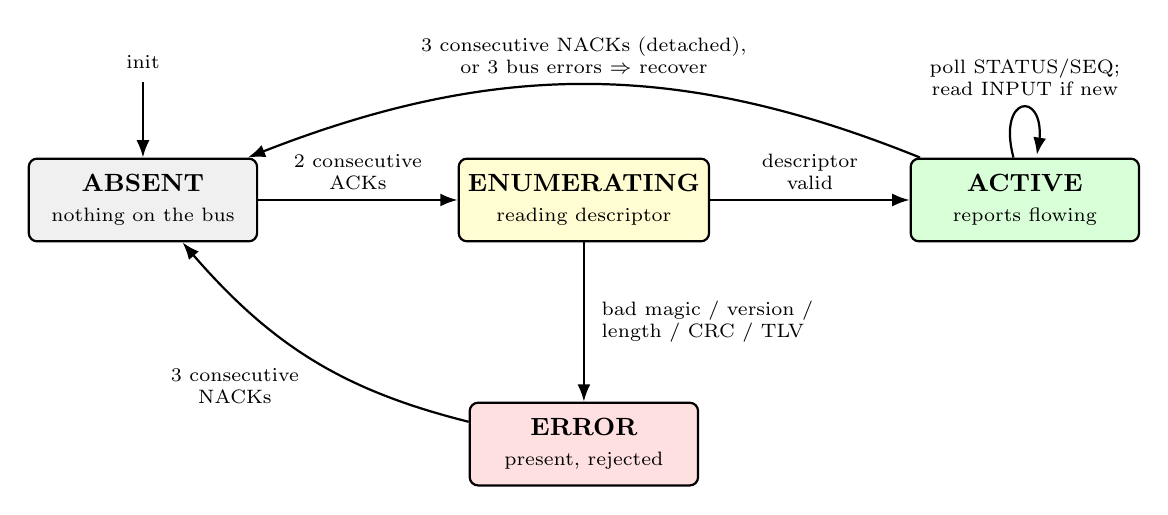
\begin{tikzpicture}[
  font=\small,
  node distance=2.4cm and 3.4cm,
  st/.style={draw, thick, rounded corners=3pt, minimum width=2.9cm, minimum height=1.05cm, align=center},
  >={Latex[length=2.2mm]},
  every edge/.style={draw, thick, ->}
]

\node[st, fill=gray!12]   (absent) at (0,0)      {\textbf{ABSENT}\\{\scriptsize nothing on the bus}};
\node[st, fill=yellow!18] (enum)   at (5.6,0)    {\textbf{ENUMERATING}\\{\scriptsize reading descriptor}};
\node[st, fill=green!15]  (active) at (11.2,0)   {\textbf{ACTIVE}\\{\scriptsize reports flowing}};
\node[st, fill=red!12]    (error)  at (5.6,-3.1) {\textbf{ERROR}\\{\scriptsize present, rejected}};

\draw (absent) edge node[above, align=center, font=\scriptsize]
  {2 consecutive\\ACKs} (enum);
\draw (enum) edge node[above, align=center, font=\scriptsize]
  {descriptor\\valid} (active);
\draw (enum) edge node[right, align=left, font=\scriptsize]
  {\ bad magic / version /\\ \ length / CRC / TLV} (error);

\draw (active) edge[bend right=22] node[above, align=center, font=\scriptsize]
  {3 consecutive NACKs (detached),\\or 3 bus errors $\Rightarrow$ recover} (absent);
\draw (error) edge[bend left=18] node[below left, align=center, font=\scriptsize]
  {3 consecutive\\NACKs} (absent);

\draw[->, thick] (absent) ++(0,1.5) -- (absent.north);
\node[font=\scriptsize] at (0,1.75) {init};

\draw (active) edge[loop above] node[above, align=center, font=\scriptsize]
  {poll STATUS/SEQ;\\read INPUT if new} (active);

\end{tikzpicture}
\caption{Host-side enumeration state machine. Attachment requires two consecutive address ACKs and detachment three consecutive NACKs, debouncing pogo-contact bounce in both directions. A module whose descriptor fails validation lands in ERROR and is not retried until it is physically removed, so a broken module cannot trap the host in a re-enumeration loop.}
\label{fig:fsm}
\end{figure}
Once the module enters the ACTIVE state, every polling cycle reads the \texttt{STATUS} and \texttt{SEQ} registers together in a single two-byte transaction. \\
We only fetch a new input report if the \texttt{DATA\_READY} bit is set and the sequence number (\texttt{SEQ}) is different from the last one we saw. \\
This way, if a module has nothing new to say, it only costs us two bytes on the bus instead of reading a full report. \\
We copy these reports into a buffer protected by a mutex, since the UI thread reads them at the exact same time the expansion thread is writing them.\\\\
We also count bus errors separately from normal \nameref{prot:i2c} NACKs. \\
If we hit three consecutive bus errors while active, we trigger Zephyr's \texttt{i2c\_recover\_bus()} function. \\
This sends clock pulses to recover a target that is stuck holding the SDA line low, and then we reset the port to ABSENT. \\
This directly answers requirement R10 and handles the open-drain hazard we mentioned in Section~\ref{sec:background}: if someone rips a module off right in the middle of a transaction, it jams the bus, so our port needs to be able to un-jam itself without forcing the user to reboot the watch.
\newpage
\subsection{Adaptive polling policy}
\label{sec:fwmp:poll}

Because we rely on polling to detect both module presence and incoming data, the polling interval dictates our entire power-versus-latency trade-off for the expansion port. The underlying principle is well established in the sensor-network literature: where a link cannot be made cheaper per transfer, the remaining lever is to make fewer transfers, by aggregating or bundling payloads and by letting the node decide locally when a transfer is worth making. Liu et al.~\cite{liu2024} formalise this as a data-collection problem and show the gain comes from bundling rather than from any change to the radio itself, and \v{S}oli\'{c} et al.~\cite{solic2024} demonstrate the same effect in a BLE health sensor, where computing a derived quantity on the node instead of streaming raw accelerometer samples is what produces the saving. We handle this in FWMP by using three different polling regimes, which are summarized below:

\begin{table}[H]
\centering
\small
\begin{tabular}{@{}l r p{8.2cm}@{}}
\toprule
\textbf{Regime} & \textbf{Interval} & \textbf{When} \\
\midrule
Absent   & \SI{1000}{\milli\second} & No module attached. One zero-length transaction per second is the standing cost of supporting expansion at all \\
Background & \SI{250}{\milli\second} & Module attached but its screen is not visible \\
Foreground & \SI{50}{\milli\second} & User is looking at the module screen; bounded below by the host, and lengthened to the module's \texttt{poll\_hint\_ms} if the module asks for something slower \\
\bottomrule
\end{tabular}
\caption{Adaptive poll intervals. The host honours a module's requested rate only in the direction that saves power: a module may ask to be polled \emph{less} often than \SI{50}{\milli\second}, never more.}
\label{tab:poll}
\end{table}
The way we handle \texttt{poll\_hint\_ms} asymmetrically is another example of our trust boundary. \\
Since this hint is data supplied by the module, we only let it influence the host's behavior when a malicious or buggy value is harmless. \\
If a module claims it needs to be polled every single millisecond, it would completely drain the watch's battery, so we clamp that request. \\
On the other hand, if a module asks to be polled every two seconds, honoring that request costs us nothing.

\subsection{Writing a compliant module}

The full contract for building a third-party module is short enough that we can state it all in one place:

\begin{enumerate}[label=\textbf{M\arabic*.}]
  \item Act as an \nameref{prot:i2c} target at 7-bit address \texttt{0x42}, \SI{3.3}{\volt} logic, up to \SI{400}{\kilo\hertz}.
  \item Do not fit pull-up resistors; the watch owns them.
  \item Draw no more than the platform current allowance from pin 1.
  \item Implement the register map of Table~\ref{tab:regmap}, readable with the write-offset/repeated-START idiom.
  \item Serve a descriptor whose magic is \texttt{`FW'}, whose version is \texttt{0x01}, whose \texttt{DESC\_LEN} is truthful and $\le$ 128, and whose final two bytes are a CRC-16/CCITT (init \texttt{0xFFFF}) over all preceding bytes.
  \item Declare at least a \texttt{NAME} TLV, plus \texttt{INPUT\_REPORT} and/or \texttt{OUTPUT\_REPORT} matching the \texttt{CAPS} bits actually set.
  \item Increment \texttt{SEQ} on every new input report and set \texttt{DATA\_READY} in \texttt{STATUS}; clear it when the report has been read.
  \item Tolerate being polled at any rate between \SI{50}{\milli\second} and \SI{1}{\second}, and tolerate power being removed at any instant.
\end{enumerate}
Nothing in this checklist requires anything more powerful than a basic 8-bit microcontroller with an \nameref{prot:i2c} peripheral. \\
That was exactly our design target: we wanted the barrier to entry for making a FinWatch module to be a weekend project, not a full-blown development contract. \\
You can find our reference module design built against this exact checklist in Appendix~\ref{app:module}.

\subsection{Summary}

To wrap up, FWMP v1 meets our expansion requirements (R8--R10) by using a four-contact interface, a fixed address, and a CRC-protected self-describing descriptor. \\
The key takeaway is that an unknown module becomes completely usable without any host-side code, while our strict bounds-checking ensures the watch remains safe from malformed or malicious module data.

\newpage
% =================================================================
\section{Implementation}
\label{sec:impl}

\subsection{Schematic capture}
Once we finalized the system design, we moved to KiCad to capture the schematic. \\
We wired up all the components to their correct operating voltages and matched every part to its appropriate protocol interface. \\
The full design is saved in the \texttt{watch\_thing\_alt.kicad\_sch} file. \\
Figures~\ref{fig:sch_power}, \ref{fig:sch_mcu}, \ref{fig:sch_periph} and~\ref{fig:sch_io} break down the schematic into functional blocks -- the PMIC power tree, the nRF5340 core with its RF front end, the peripherals, and the external pogo-pin I/O with its level shifter. \\
The official KiCad exports are attached in Appendix~\ref{app:hw}.

% ---------------------
\begin{figure}[H]
\centering
\begin{circuitikz}[american, transform shape, scale=0.82, font=\footnotesize]
    % QSPI flash
    \node[draw, thick, minimum width=3.4cm, minimum height=2.4cm] (U2) at (0,0){};
    \node[font=\bfseries] at ([yshift=-5mm]U2.north){U2};
    \node[font=\scriptsize] at (U2.center){MX25U51245G};
    \node[font=\scriptsize] at ([yshift=5mm]U2.south){512\,Mb QSPI flash};
    \draw (U2.north) -- ++(0,0.9) coordinate(f18) node[above]{+1.8V};

    % decoupling capacitor
    \draw (f18) -- ++(3.6,0) to[C, l=\SI{0.1}{\micro\farad}, a=$C26$] ++(0,-1.8) node[ground]{};
    \draw (U2.south) -- ++(0,-0.3) node[ground]{};
    \draw (U2.west) -- ++(-2,0) node[above left]{\ttfamily QSPI \; P0.13--P0.18};

    % IMU
    \node[draw, thick, minimum width=3.4cm, minimum height=2.4cm] (U3) at (0,-5.5){};
    \node[font=\bfseries] at ([yshift=-5mm]U3.north){U3};
    \node[font=\scriptsize] at (U3.center){LSM6DSOX};
    \node[font=\scriptsize] at ([yshift=5mm]U3.south){6-axis IMU};
    \draw (U3.north) -- ++(0,0.9) coordinate(i18) node[above]{+1.8V};
    % decoupling capacitor
    \draw (i18) -- ++(3.6,0) to[C, l=\SI{0.1}{\micro\farad}, a=$C27$] ++(0,-2.8) node[ground]{};
    \draw (U3.south) -- ++(0,-0.3) node[ground]{};
    \draw ([yshift=5mm]U3.west) coordinate(sda) -- ++(-3.6,0) node[above left]{\ttfamily ACC SDA \; P1.13};
    \draw ([yshift=-1mm]U3.west) coordinate(scl) -- ++(-3.6,0) node[above left]{\ttfamily ACC SCL \; P1.12};
    \draw ([yshift=-7mm]U3.west) -- ++(-3.6,0) node[above left]{\ttfamily INT1/INT2 \; P1.14/P1.15};
    \draw (sda) ++(-1.3,0) node[circ]{} to[R, l=\SI{4.7}{\kilo\ohm}, a=$R10$] ++(0,2.4) coordinate(t10);
    \draw (scl) ++(-2.9,0) node[circ]{} to[R, l_=\SI{4.7}{\kilo\ohm}, a^=$R11$] ++(0,3.0) coordinate(t11);
    \draw (t11) -- (t10) node[midway, above=1pt]{+1.8V};

    % LCD / touch connector
    \node[draw, thick, minimum width=3.4cm, minimum height=2.6cm] (J2) at (0,-9.5){};
    \node[font=\bfseries] at ([yshift=-4mm]J2.north){J2 \; ($1\times13$)};
    \node[font=\scriptsize, align=center] at ([yshift=5mm]J2.south){Waveshare LCD\\+ touch};
    \draw ([yshift=8mm]J2.west) -- ++(-3.4,0) node[above left]{\ttfamily LCD SPI \; P0.8--P0.12};
    \draw ([yshift=1mm]J2.west) -- ++(-3.4,0) node[above left]{\ttfamily Touch I\textsuperscript{2}C \; P0.23/P0.24};
    \draw ([yshift=-7mm]J2.west) -- ++(-3.4,0) node[above left]{\ttfamily RST/DC/BL/INT};
    \draw (J2.east) -- ++(1,0) node[above right]{+3.3V (BL)};
\end{circuitikz}
\caption{Peripherals. The QSPI flash (U2) and LSM6DSOX IMU (U3) run from the \SI{1.8}{\volt} rail, each with a local \SI{0.1}{\micro\farad} decoupling capacitor; R10/R11 pull up the accelerometer \nameref{prot:i2c} bus. The SPI display and its capacitive-touch controller share connector J2.}
\label{fig:sch_periph}
\end{figure}

% ---------------------
\begin{figure}[H]
\centering
\begin{circuitikz}[american, transform shape, scale=0.78, font=\footnotesize]
    % Level shifter
    \node[draw, thick, minimum width=3cm, minimum height=3.4cm] (U6) at (0,0){};
    \node[font=\bfseries] at ([yshift=-5mm]U6.north){U6};
    \node[font=\scriptsize] at (U6.center){PCA9306};
    \node[font=\scriptsize, align=center] at ([yshift=7mm]U6.south){I\textsuperscript{2}C level shift\\ $1.8\,\text{V}\leftrightarrow3.3\,\text{V}$};

    % Low (1.8 V) side
    \draw ([yshift=9mm]U6.west) coordinate(lscl) -- ++(-3.8,0) node[above left]{\ttfamily PERIPH SCL \; P0.30};
    \draw ([yshift=1mm]U6.west) coordinate(lsda) -- ++(-3.8,0) node[above left]{\ttfamily PERIPH SDA \; P0.31};
    \draw (lscl) ++(-1.3,0) node[circ]{} to[R, l=\SI{4.7}{\kilo\ohm}, a=$R2$] ++(0,2.4) coordinate(tl1);
    \draw (lsda) ++(-2.9,0) node[circ]{} to[R, l_=\SI{4.7}{\kilo\ohm}, a^=$R3$] ++(0,3.21) coordinate(tl2);
    \draw (tl2) -- (tl1) node[midway, above=1pt]{+1.8V};

    % High (3.3 V) side
    \draw ([yshift=9mm]U6.east) coordinate(hscl) -- ++(2.8,0) coordinate(j1a);
    \draw ([yshift=1mm]U6.east) coordinate(hsda) -- ++(2.8,0) coordinate(j1b);
    \draw (hscl) ++(1.3,0) node[circ]{} to[R, l=\SI{4.7}{\kilo\ohm}, a=$R4$] ++(0,2.4) coordinate(th1);
    \draw (hsda) ++(2.6,0) node[circ]{} to[R, l_=\SI{4.7}{\kilo\ohm}, a^=$R5$] ++(0,3.21) coordinate(th2);
    \draw (th1) -- (th2) node[midway, above=1pt]{+3.3V};

    % Pogo \nameref{prot:i2c} header
    \node[draw, thick, minimum width=2cm, minimum height=2.4cm] (J1) at (6.6,0.5){};
    \node[font=\bfseries] at ([yshift=-4mm]J1.north){J1};
    \node[font=\scriptsize, align=center] at ([yshift=5mm]J1.south){4-pin pogo\\ext.\ I\textsuperscript{2}C};
    \draw (j1a) -- (J1.west|-j1a);
    \draw (j1b) -- (J1.west|-j1b);
    \draw ([yshift=7mm]J1.east) -- ++(0.8,0) node[above right]{+3.3V};
    \draw ([yshift=-7mm]J1.east) -- ++(0.8,0) node[below right]{GND};

    % USB / charge pogo header
    \node[draw, thick, minimum width=2cm, minimum height=3cm] (J3) at (6.2,-4.6){};
    \node[font=\bfseries] at ([yshift=-4mm]J3.north){J3};
    \node[font=\scriptsize, align=center] at ([yshift=6mm]J3.south){6-pin pogo\\USB / charge};
    \draw ([yshift=11mm]J3.west) -- ++(-4,0) node[above left]{VBUS $\to$ U4};
    \draw ([yshift=3mm]J3.west)  -- ++(-4,0) node[above left]{\ttfamily D+ / D- \; (U1)};
    \draw ([yshift=-4mm]J3.west) -- ++(-4,0) node[above left]{\ttfamily CC1 / CC2 \; (U1)};
    \draw ([yshift=-11mm]J3.west) -- ++(-4,0) node[above left]{GND};

    % User buttons
    \draw (-7.2,-7) node[ground]{} to[push button, l=$SW2$] ++(2.6,0) node[above right]{\ttfamily P1.0 (BTN1)};
    \draw (-7.2,-8.6) node[ground]{} to[push button, l=$SW3$] ++(2.6,0) node[above right]{\ttfamily P1.1 (BTN2)};
\end{circuitikz}
\caption{External I/O. The PCA9306 (U6) translates the nRF5340 \SI{1.8}{\volt} \texttt{PERIPH} \nameref{prot:i2c} bus to \SI{3.3}{\volt} on the J1 pogo header, with pull-ups R2/R3 on the low side and R4/R5 on the high side, the electrical contract of Table~\ref{tab:j1}. J3 carries USB \texttt{VBUS}, \texttt{D+/D-} and the USB-C \texttt{CC1/CC2} lines used for charging. SW2/SW3 are the user push-buttons on P1.0/P1.1.}
\label{fig:sch_io}
\end{figure}

\subsection{PCB layout}
After finishing the schematic, we tackled the PCB layout. \\
We strictly applied the design principles we discussed back in Section~\ref{sec:background}. \\
We placed the decoupling capacitors as close as physically possible to their respective supply pins, kept the switching loops of the buck converters tight around the PMIC, ensured an uninterrupted ground return path under every signal, and kept all copper out of the antenna region.

\begin{table}[H]
\centering
\small
\begin{tabular}{@{}l l@{}}
\toprule
\textbf{Parameter} & \textbf{Value} \\
\midrule
Board outline & Circular, \SI{45.97}{\milli\metre} diameter \\
Layer count & 4 (\texttt{F\_Cu}, \texttt{In1\_Cu}, \texttt{In2\_Cu}, \texttt{B\_Cu}) \\
Board thickness & \SI{1.0}{\milli\metre}, FR-4 \\
Copper weight & \SI{1}{oz} outer, \SI{0.5}{oz} inner \\
Surface finish & ENIG (immersion gold) \\
Solder mask / silkscreen & Green / white \\
Minimum drill & \SI{0.15}{\milli\metre} (27 holes) \\
Drill classes & 0.15, 0.20, 0.30, \SI{0.50}{\milli\metre} plated; 0.90, \SI{2.10}{\milli\metre} non-plated \\
Total holes & 170 (164 plated, 6 non-plated) \\
Via treatment & Epoxy filled and capped (IPC-4761 Type VII) \\
Component count & 30 BOM lines, 88 placements \\
Manufacturer / process & JLCPCB, 4-layer FR-4 with resin via fill \\
Panelisation & \SI{71.97}{\milli\metre} square panel, \SI{13}{\milli\metre} process rails \\
\bottomrule
\end{tabular}
\caption{PCB physical parameters, as confirmed against the manufacturer's CAM output.}
\label{tab:pcb}
\end{table}

\subsubsection{Via-in-pad and the cost of fine-pitch escape routing}
\label{impl:viainpad}

The nRF5340 comes in an aQFN-94 package, which squeezes 94 pads onto a \SI{0.4}{\milli\metre} grid inside a $7\times7\,\text{mm}$ body with a central thermal pad. \\
Routing all these signals out was easily the hardest layout challenge on the board, and it's what ultimately dictated our layer count, minimum drill size, and overall manufacturing process.

\paragraph{Why the conventional escape fails.} The standard \emph{dog-bone} technique -- routing a short trace from the pad to a via placed in the empty space between the pads -- simply fails here. \\
At a \SI{0.4}{\milli\metre} pitch, that space just does not exist. \\
Even using a tiny \SI{0.15}{\milli\metre} drill with a minimum annular ring and standard clearance rules, there is no physical width left for the escape trace. \\
We could only escape the outer row or two, leaving the inner rows completely unreachable.

\paragraph{Via-in-pad.} The only working solution is placing the via directly inside the component pad, dropping the signal straight to an inner layer so no escape trace is needed. \\
We placed 25 vias (\SI{0.15}{\milli\metre}) exactly on the package's \SI{0.4}{\milli\metre} grid inside the pads of U1. \\
Every single one sits perfectly dead-center in its pad, perfectly aligned with the solder-paste aperture and solder-mask opening. \\
However, via-in-pad is not free -- you just pay for it in manufacturing instead of layout. An open via is basically a hole beneath molten solder. \\
During reflow, capillary action will suck the solder down the barrel and away from the joint. This leaves an unpredictable, starved, or voided connection under a package that we can't even inspect without an X-ray machine. \\
To prevent this, the via has to be filled and leveled before the board is ever assembled.

\paragraph{The filled-and-capped process.} Our board required the IPC-4761 Type VII filled-and-capped treatment, which forces the fabricator to inject several extra steps right in the middle of normal production:

\begin{enumerate}
  \item Drill and plate the vias as usual to form the copper barrel.
  \item Fill each barrel with a non-conductive epoxy resin under a vacuum, making absolutely sure no air gets trapped.
  \item Cure the resin.
  \item Planarize the board by grinding the surface flush, removing any excess resin that sticks out above the copper.
  \item Plate a solid copper ``cap'' over the filled via to close it up and restore a perfectly flat, solderable pad.
  \item Continue with the standard outer-layer imaging, solder mask, and surface finish.
\end{enumerate}
The consequences of this process for a project of our scale are worth spelling out, mainly because they are completely invisible in the layout files:

\begin{itemize}
  \item \textbf{Cost.} Via filling comes with a per-order surcharge, and the \SI{0.15}{\milli\metre} drills triggered a ``small-hole'' fee as well. We were charged for both on this order.
  \item \textbf{Lead time.} Because these four extra steps (fill, cure, planarize, cap) happen in the middle of fabrication, you cannot expedite the board past them.
  \item \textbf{Supplier choice.} Not every low-cost board house offers resin fill with cap plating. Requiring it immediately narrowed down our options before we even asked for quotes, which tied directly into the procurement headaches we discuss in Section~\ref{sec:challenges}.
  \item \textbf{Failure modes move upstream.} If the manufacturer leaves air or moisture in the via, it will outgas during reflow and literally blow out the joint above it. If they over-grind or under-plate the cap, it leaves a dimple that ruins the pad's coplanarity. We cannot see or fix either of these issues after assembly, so our design relies entirely on the fabricator's process control rather than anything we can verify in the lab.
\end{itemize}
It is worth noting that none of this was strictly forced by the application itself. \\
If we had used a pre-certified module with the same SoC, we would have had coarse-pitch pads that route easily on two layers without any via-in-pad at all (and comparable projects take exactly that route, as discussed in Section~\ref{sec:discussion}). \\
We consciously paid the price of using bare silicon to save board area, reduce unit costs, and take full ownership of the RF design and escape routing.\\\\
The general lesson here is that choosing a \SI{0.4}{\milli\metre}-pitch package isn't just a routing decision -- it transfers a big chunk of the board's reliability from the layout phase, where we can check it, to the fabricator's floor, where we can't. \\
Having chosen bare silicon for a board that has to fit inside a watch case, no coarser-pitch package was a realistic alternative, but we made the trade-off knowingly. \\
This is exactly why we went through the manufacturer's CAM files hole-by-hole before production.\\\\
In addition, we made a few important layout decisions that are not obvious from the schematic. \\
\begin{enumerate}
  \item We placed the PMIC and its two inductors in a tight cluster in the middle of the board, so the switching loops are as small as possible and the EMI is contained.
  \item We placed the IMU near the board center so its axes are consistent regardless of how the watch is worn.
  \item We placed the antenna at the board edge with a keepout zone around it, and routed the RF match as a controlled-impedance line.
  \item We routed the \SI{1.8}{\volt} and GND power planes on the inner layers to ensure there was a short return path for the high-frequency signals.
  \item We used a 4-layer stackup to allow for better routing of the high-density signals and to provide a solid ground reference for the RF signals.
\end{enumerate}

\subsection{Mechanical design}
To house the electronics, we designed a custom enclosure in Fusion 360. \\
The enclosure is designed to be 3D printed, with a window on the left side and below to allow for pogo pin connection. \\
Note: altough the render shows the first revision of the watch, the final design has the same window placement and the same overall dimensions. \\
\begin{figure}[H]
\centering
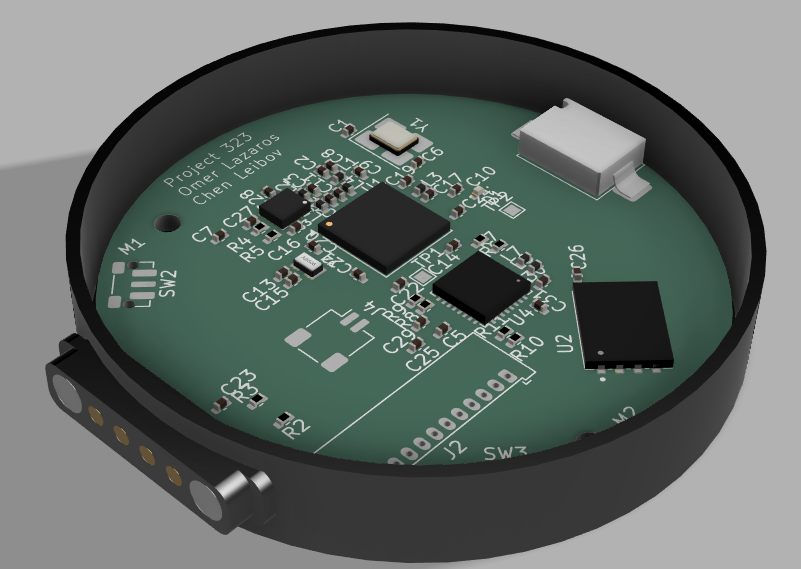
\includegraphics[width=0.8\textwidth]{images/watch_render.png}
\caption{Render of the watch enclosure in fusion, there is a window both on the left side and below to allow for pogo pin connection, the display should cover the opening up top.}
\label{fig:watch_render}
\end{figure}

\subsection{Firmware}

We wrote the firmware targeting the nRF5340 application core using the Zephyr RTOS and the nRF Connect SDK. To keep things organized, we divided the code into nine separate subsystems. Each subsystem sits in its own directory under \texttt{src/} and exposes a minimal header file to the rest of the application.

\begin{table}[H]
\centering
\small
\begin{tabular}{@{}l r p{8.4cm}@{}}
\toprule
\textbf{Subsystem} & \textbf{LOC} & \textbf{Responsibility} \\
\midrule
\texttt{expansion/} & 915 & FWMP host: transport, protocol, state machine, mock backend \\
\texttt{display/}   & 593 & LVGL setup, watch face, module screen, test screen \\
\texttt{sensor/}    & 395 & LSM6DSOX wake-up interrupt, active-window sampling, step detection \\
\texttt{ble/}       & 294 & GATT services, advertising, battery notification \\
\texttt{main.c}     & 178 & Subsystem init, button handling, 1\,Hz update thread \\
\texttt{rtc/}       & 115 & Timekeeping \\
\texttt{storage/}   & 110 & File system on QSPI flash, settings persistence \\
\texttt{buttons/}   & 78  & Debounce, short/long press classification \\
\texttt{touch/}     & 73  & Capacitive touch controller, LVGL input device \\
\texttt{pmic/}      & 58  & nPM1300 battery percentage and charge state \\
\midrule
\textbf{Total}      & \textbf{2\,809} & \\
\bottomrule
\end{tabular}
\caption{Firmware size by subsystem (lines of C, headers included). The expansion port is the largest single subsystem in the project, roughly a third of the codebase, which reflects that it is the contribution rather than the plumbing.}
\label{tab:loc}
\end{table}

\paragraph{Hardware abstraction.} Following the design principles we mentioned in Section~\ref{sec:background}, we didn't hardcode any GPIO pins, bus frequencies, or \nameref{prot:i2c} addresses of on-board devices into our C code. \\
Everything is resolved cleanly from the Devicetree. \\
However, we made one deliberate exception: the expansion module itself. \\
Since the module is hot-plugged hardware that might not even be attached when the watch boots, it doesn't get a Devicetree node. \\
Declaring a child node for a device that is usually absent is a misuse of the Devicetree model. \\
Instead, our transport layer takes the \nameref{prot:i2c} bus controller (\texttt{i2c3}) from the Devicetree and addresses \texttt{0x42} directly.

\paragraph{Transport abstraction and the mock backend.} We split the expansion subsystem so our protocol logic never has to touch Zephyr's \nameref{prot:i2c} API directly. \\
We declared five basic operations (init, probe, read, write, recover) and built two backends: the real \nameref{prot:i2c} hardware backend, and a mock backend. \\
The mock backend simulates a ``Test Dial'' module with a rotating input report and can intentionally inject six different classes of fault on demand -- five kinds of malformed descriptor and a bus error. \\
Building this mock allowed us to fully test the protocol logic without any physical module hardware, and it serves as the foundation for our fault-injection tests in Section~\ref{sec:results}.

\paragraph{Interrupt-driven motion wake.}
\label{impl:wake}
To satisfy requirement R5, we had to make sure the host doesn't continuously poll the IMU. \\
We shifted the responsibility of detecting motion from the CPU directly to the sensor. \\
The BMI270 has a built-in wake-up function that compares the acceleration slope against a programmable threshold and asserts the INT1 pin when that threshold is crossed. \\
We configure this directly over \nameref{prot:i2c} because the standard Zephyr driver only gives us a ``data-ready'' trigger. \\
Using a data-ready trigger would wake the CPU for every single sample, which completely defeats the purpose of putting the MCU to sleep. \\
This is the wearable-scale version of a result \v{S}oli\'{c} et al.~\cite{solic2024}
report for a BLE health sensor: computing a derived quantity on the node, and
reporting only that, costs far less than moving every raw sample to wherever the
decision is made. \\
Therefore, we left the Zephyr trigger unconfigured so the driver doesn't claim the interrupt line, and let our custom sensor subsystem take full ownership of it.

This setup creates a clean, two-state control flow:

\begin{itemize}
  \item \textbf{Idle.} The sensor thread blocks indefinitely on a semaphore. It consumes zero CPU time and generates absolutely no timer wake-ups, while the IMU automatically drops into a \SI{12.5}{\hertz} low-power mode.

  \item \textbf{Active.} When the INT1 pin fires, the interrupt service routine (ISR) releases the semaphore. The thread wakes up, reads the \texttt{WAKE\_UP\_SRC} register to confirm a genuine motion event, wakes the display, and starts sampling at \SI{10}{\hertz} for step detection. \\
  The active window closes \SI{3}{\second} after the last motion event (or immediately if the sensor reports inactivity), and the thread goes right back to sleep.
\end{itemize}
%
We don't lose any step data by only sampling inside this active window, because steps literally only happen when the wrist is moving.\\
The underlying idea --- let the sensor decide when the host is needed, and spend
energy in proportion to what is actually happening --- is the same one Chen and
Rodriguez-Villegas~\cite{chen2025} use to keep a wristband running without a
battery at all, where the sampling rate is driven by the signal and the
harvesting conditions rather than by a fixed schedule. Our version is far more
modest: a single threshold and one active window, on a device that still has a
cell to fall back on.\\
We configured the interrupt as latched, meaning we have to acknowledge it by reading the source register. \\
If we miss an acknowledgment, the INT1 line stays high and silently kills the entire wake-up path. \\
To prevent this, we read the source register on every single event and every time we exit the active window. \\
We also built in a fail-safe: if the interrupt fails to initialize (like if the pin isn't wired properly on a bench setup), the firmware logs a warning and falls back to continuous \SI{10}{\hertz} polling. \\
This ensures the step counter still works, but it degrades the battery life.
%

\paragraph{Toolchain and dependencies.}
\begin{itemize}
  \item Zephyr RTOS 4.4.0 via nRF Connect SDK 3.2.1
  \item Arm GNU toolchain, built with \texttt{west}
  \item LVGL for the user interface
  \item KiCad 10.0 for schematic and PCB
  \item Autodesk Fusion for the enclosure
\end{itemize}

% =================================================================
\section{Design challenges and revisions}
\label{sec:challenges}

This section goes over the main problems we ran into that ended up shaping the final design. We are explicitly documenting our Revision A defect here, not because it is flattering, but because the debugging process and the checklist it generated are actual, valuable results of this project.

\subsection{Revision A defect: no debug access}

\paragraph{Symptom.} We manufactured and assembled the first PCB revision. The power rails came up correctly, but the board was completely unprogrammable -- we couldn't load firmware or debug it at all.

\paragraph{Root cause.} We simply forgot to route the nRF5340's \texttt{SWDIO} and \texttt{SWDCLK} pins in the schematic. Since a blank nRF5340 has no bootloader, the Serial Wire Debug (SWD) interface is the only way to flash the very first image. Omitting it essentially rendered the board permanently unprogrammable. This mistake slipped right past our design review because SWD isn't a functional net for any other component on the board. An Electrical Rules Check (ERC) only verifies the connections you actually drew; it cannot warn you about connections that should exist but don't.

\paragraph{Fix.} In Revision B, we routed the three debug signals out to $1.0\times1.0\,\text{mm}$ test pads on the board surface: \texttt{SWDIO} to TP4, \texttt{SWDCLK} to TP3, and \texttt{nRESET} to TP2. We used test pads instead of a physical header to save board area and enclosure volume, which is critical for a watch. We also made sure to include the \texttt{nRESET} line. If faulty firmware locks up the core, a simple two-pad SWD setup won't let the debugger halt the device, so you absolutely need the reset line to make the debug interface robust.

\paragraph{Lesson and process change.} This failure directly led us to create a strict pre-fabrication checklist (Section~\ref{sec:challenges:checklist}) to manually verify all the critical nets that automated rules checks miss.

\subsection{Component availability}

During the project, supply chain shortages affected both our PMIC and our IMU.

\paragraph{PMIC shortage.} The nPM1300 PMIC we specified was out of stock at every distributor we checked, and the lead time quoted by the manufacturer was longer than our remaining project schedule. We had to switch to a different PMIC (the nPM1100) that was in stock and could be delivered on time.\\
Since the npm1300 uses a unique package and pinout, we couldn't just swap the part, we had to wait and check all of the leading distributors for stock, until we found one that could deliver the part in time.


\paragraph{Procurement as a design constraint.} We learned firsthand that procurement is a strict design constraint. \\
Several suppliers refused to even quote us for the single-unit quantities a student project requires, and others quoted lead times longer than our remaining project schedule. \\
We even had one order canceled outright after it was placed due to an administrative error on the supplier's side, which cost us a further 14 weeks before we could arrange an alternative.\\\\
These issues had two direct consequences for our design. \\
First, the part we specified wasn't always the part we could obtain. \\
Second, availability stopped being just a procurement detail and became a core selection criterion alongside the technical specs in Table~\ref{tab:selection}. \\
A part with a unique footprint and no compatible alternate carries a massive schedule risk. \\
This reality is invisible in the finished hardware, but it is a major difference between our student prototype and a commercial product backed by real purchasing power and supplier relationships.

\paragraph{Lesson.} In a student project with a single fabrication opportunity, second-source availability deserves to be a primary selection criterion. \\
Our IMU substitution showed exactly what makes a second source genuinely usable rather than merely similar: because the replacement was pin-for-pin compatible, the board needed absolutely no changes. \\
Because our hardware dependencies were isolated in the Devicetree, the software change needed for the substitution itself was confined to an overlay node and a driver selection (the interrupt-driven wake path added later, Section~\ref{impl:wake}, does program LSM6DSOX registers directly). \\
If we had hardcoded the sensor's address and register map into our C code, or used a part with a unique pinout, this exact same shortage would have forced us to do a full board re-spin.

\subsection{The two-voltage-domain problem}

The nRF5340 operates its I/O at \SI{1.8}{\volt}, but essentially every peripheral a user might attach (and the display backlight) expects \SI{3.3}{\volt}. We evaluated three options:

\begin{enumerate}
  \item Run the entire board at \SI{3.3}{\volt}. (Rejected: it raises the switching power of every digital transition on the board, and the MX25U51245G external flash is a \SI{1.8}{\volt}-only part.)
  \item Expose the expansion port at \SI{1.8}{\volt} and require modules to match. (Rejected: makes the port useless for the target audience, since off-the-shelf sensor breakouts run at \SI{3.3}{\volt}.)
  \item Keep the digital domain at \SI{1.8}{\volt} and translate at the boundary. (Chosen.)
\end{enumerate}

We went with option 3. This cost us one PCA9306 level shifter and a second pair of pull-up resistors. The PCA9306 strictly relies on pull-ups on both sides to function, so the resistor pairs aren't redundant duplicates --- they are required. This is exactly why we explicitly forbid external modules from incorporating their own pull-ups (rule M2 in Section~\ref{sec:fwmp}).

\subsection{No interrupt line on the expansion port}

As discussed in Section~\ref{sec:fwmp}, we rejected adding a fifth pogo contact to save mechanical space. The trade-off is that our purely polled port constantly burns idle current and has a worst-case attach latency of two poll intervals. Our adaptive polling policy (Table~\ref{tab:poll}) is the mitigation for this.

\subsection{Hot-plug on an open-drain bus}

If a user unplugs a module mid-transaction, it can leave the SDA line held low, which jams the bus until it is recovered. This isn't hypothetical; it's exactly what can happen when physical contacts are disconnected unexpectedly. To handle this, the host explicitly counts consecutive bus errors separately from normal NACKs. If it hits three errors, it calls Zephyr's \texttt{i2c\_recover\_bus()} to send clock pulses and un-jam the line, resetting the port back to the ABSENT state without requiring a hard reboot.

\subsection{Storage subsystem partition-ID collision}

During our DK bring-up, mounting the file system caused a SecureFault instead of a graceful failure. The fixed-partition ID we used for our external QSPI flash collided with the DK's internal \texttt{storage\_partition}. Since the external flash isn't populated on the DK, the mount should have just failed so the boot could continue. We temporarily disabled storage initialization in \texttt{main()} until we have the real flash hardware on Revision B.\\
This was added back to the final board.

\subsection{Pre-fabrication design-review checklist}
\label{sec:challenges:checklist}

Derived from all the problems above, this is the checklist we now apply before releasing a board revision:

\begin{enumerate}[label=\textbf{C\arabic*.}]
  \item Is SWD (\texttt{SWDIO}, \texttt{SWDCLK}, \texttt{nRESET}, reference ground, target voltage) brought out to an accessible connector or pad set?
  \item Does every power rail have a test point, and is there at least one ground clip point?
  \item Has ERC been run with no unexplained warnings, \emph{and} has a human separately verified the nets ERC cannot know about (debug, straps, unused-pin termination)?
  \item Has DRC been run clean against the manufacturer's actual capabilities, not the default profile?
  \item Is every part on the BOM in stock, from at least two distributors, with a documented second source?
  \item For each critical part, is there a functionally equivalent alternate in the \emph{same footprint}, so that a substitution costs a BOM line rather than a board revision?
  \item Have quoted lead times and minimum order quantities been checked against the remaining project schedule, with the order placed early enough to absorb one cancellation?
  \item Does every IC have local decoupling placed on the same layer and within a few millimetres of its supply pin?
  \item Is the antenna keepout free of copper on all layers, and is the RF match routed as a controlled-impedance line?
  \item Have the mechanical outline, connector positions, and mounting holes been checked against the enclosure model?
\end{enumerate}

\newpage
% =================================================================
\section{Verification and results}
\label{sec:results}

We verified our system on three main fronts, based on what hardware was available at the time. We ran functional verification of the firmware on the nRF5340-DK, electrical verification on our manufactured Revision A board, and fault-injection testing on the expansion protocol using our mock transport. For each experiment below, we outline the objective, the method, the results, and exactly what those results do and don't prove.

\subsection{Experiment 1: Functional verification on the nRF5340-DK}

\paragraph{Objective.} We wanted to prove that the complete firmware --- including the display, touch, sensor, BLE, buttons, and FWMP host --- works correctly regardless of the custom board.

\paragraph{Method.} We compiled the firmware for the nRF5340-DK target and tested it manually against a smartphone acting as the BLE central. Because Zephyr abstracts the hardware into the Devicetree, we were able to run the exact same application code on the DK that we will eventually use on the custom board.

\paragraph{Results.} The display renders watch face, touch registers input, BLE advertises and a central connects and receives battery
notifications, buttons produce short/long events. State which subsystems were
not verifiable on the DK, external QSPI flash is not populated, so storage
was disabled; the PMIC is absent, so battery percentage is not meaningful.

\paragraph{Interpretation.} This confirms that our application logic and FWMP host implementation are solid, even if it doesn't prove anything about the custom PCB itself. Being able to separate the software from the hardware allowed us to keep developing firmware in parallel with board fabrication.

\subsection{Experiment 2: Expansion protocol, nominal path}

\paragraph{Objective.} We needed to show that the watch can discover, enumerate, and interact with a module without having any module-specific code pre-compiled into the firmware.

\paragraph{Method.} We enabled \texttt{CONFIG\_FINWATCH\_EXPANSION\_MOCK=y} to let the mock backend simulate plugging in a fake ``Test Dial'' module. This fake module reports a vendor ID of \texttt{0xABCD}, a product ID of \texttt{0x0001}, both INPUT and OUTPUT capabilities, a 4-byte input report, a 1-byte output report, and a \SI{100}{\milli\second} requested poll interval. We triggered the attach and detach events manually using \texttt{expansion\_mock\_set\_attached()}.

\paragraph{Interpretation.} The watch successfully displayed and exchanged data with a module that it didn't know existed at compile time, strictly by reading its descriptor. This proves the core claim we made in Section~\ref{sec:fwmp} works end-to-end.

\subsection{Experiment 3: Expansion protocol, fault injection}

\paragraph{Objective.} We wanted to verify that the host safely catches every single rejection path, ensuring that a malformed descriptor can never cause the watch to crash or behave incorrectly.

\paragraph{Method.} We used the mock backend to artificially inject six different classes of faults via \texttt{expansion\_mock\_set\_fault()}. The backend rebuilds the descriptor with the chosen fault applied, and the host tries to enumerate it normally.

\begin{table}[H]
\centering
\small
\begin{tabular}{@{}l p{5.6cm} l p{3.6cm}@{}}
\toprule
\textbf{Fault} & \textbf{What is corrupted} & \textbf{Expected} & \textbf{Observed} \\
\midrule
\texttt{BAD\_MAGIC} & \texttt{MAGIC0} set to \texttt{0x00} & Reject, \texttt{ERROR} & Works as expected \\
\texttt{BAD\_VERSION} & \texttt{PROTO\_VER} set to \texttt{0x99} & Reject (\texttt{-ENOTSUP}) & Works as expected \\
\texttt{BAD\_CRC} & Trailing CRC inverted & Reject, \texttt{ERROR} & Works as expected \\
\texttt{OVERSIZE\_LEN} & \texttt{DESC\_LEN} declared as 200 ($>$ 128) & Reject before any read & Works as expected \\
\texttt{TLV\_OVERRUN} & \texttt{INPUT\_REPORT} TLV claims a 200-byte payload & Reject, no out-of-bounds read & Works as expected \\
\texttt{BUS\_ERROR} & All transactions return \texttt{-EIO} & 3 errors $\Rightarrow$ recover, $\to$ \texttt{ABSENT} & Works as expected \\
\bottomrule
\end{tabular}
\caption{Fault-injection matrix for the FWMP host. Each row corresponds to one validation step in Section~\ref{sec:fwmp:enum}; together they cover every rejection branch in the enumeration path.}
\label{tab:faults}
\end{table}

\paragraph{Interpretation.} All six faults are rejected without incorrect state transitions and without
reads past buffer bounds, and note that the OVERSIZE\_LEN and TLV\_OVERRUN cases
in particular are the ones that would be memory-safety failures in a naive
implementation.

\subsection{Experiment 4: Revision B electrical bring-up}

\paragraph{Objective.} We needed to verify that the power architecture on our manufactured Revision B board actually works as designed, since the missing debug access meant we couldn't test it with firmware.

\paragraph{Method.} We used a modified usb cable to connect to the board's USB VBUS and GND, and measured the output of the two buck converters, the ripple on each rail, the expansion port voltage, and the quiescent current. We also measured the charge current from VBUS to the battery.\\\\
Unfortunately, after many probes using a multimeter and a bench supply to bypass the usb signal, we found out that the nPM1300 PMIC was not functioning correctly, we checked all of the other connections on the board\\
we could not get the correct voltage in the board in time or fix it, therefore we could not measure the expected values in Table~\ref{tab:elec} and we could not verify the power tree. \\

\begin{table}[H]
\centering
\small
\begin{tabular}{@{}l l l l@{}}
\toprule
\textbf{Measurement} & \textbf{Expected} & \textbf{Measured} & \textbf{Pass/Fail} \\
\midrule
BUCK1 output & \SI{1.8}{\volt} $\pm$ tolerance & N/A & N/A \\
BUCK2 output & \SI{3.3}{\volt} $\pm$ tolerance & N/A & N/A \\
Expansion port pin 1 (J1) & \SI{3.3}{\volt} & N/A & N/A \\
\bottomrule
\end{tabular}
\caption{Revision-B electrical measurements.}
\label{tab:elec}
\end{table}

\subsection{Threats to validity}

\begin{itemize}
  \item \textbf{The expansion protocol was verified against a mock, not physical module hardware.}
  The mock is great for testing the host logic thoroughly (including weird faults a real well-behaved module wouldn't produce), but it doesn't simulate real-world electrical issues like contact bounce timing, clock stretching by a slow target, trace capacitance, or hot-plug brownouts.

  \item \textbf{No Revision B measurements exist yet.} Since Revision A couldn't run firmware, all our functional claims about the custom board itself are still pending.

  \item \textbf{Walking current is not the platform floor.} Even with the wake interrupt working, our step detection still runs on the application core at \SI{10}{\hertz}. Measuring current while walking will overstate the power draw compared to what the hardware would use if we offloaded step counting completely to the sensor's embedded pedometer.

  \item \textbf{Step counting was never validated against a reference.} We verified that the step detector increments while walking, which is not the same as verifying that it is accurate. Establishing that would need a reference instrument and a protocol over a population, of the kind used in the smartwatch validation study of Liu et al.~\cite{liu2025}; we make no accuracy claim.

  \item \textbf{Single-unit sample.} All our electrical measurements come from one assembled board, meaning we haven't characterized any component tolerances or assembly variations.
\end{itemize}

% =================================================================
\section{Discussion and comparison with prior work}
\label{sec:discussion}
In this section, we compare our project against existing wearable platforms and expansion ecosystems to clearly define what we actually contributed.
\subsection{Comparison with existing wearable platforms}

\begin{table}[H]
\centering
\small
\begin{tabular}{@{}l c c c c@{}}
\toprule
\textbf{Property} & \textbf{PineTime} & \textbf{Thingy:53 / DK} & \textbf{ZSWatch} & \textbf{FinWatch} \\
\midrule
Wearable form factor        & Yes & No & Yes & Yes \\
Open schematic              & Yes & Yes & Yes & Yes \\
User-replaceable firmware   & Yes & Yes & Yes & Yes \\
Dual-core radio isolation   & No & Yes & Yes & Yes \\
SoC integration             & Module & Module & Module & \textbf{Bare IC} \\
RF front end designed in-house & No & No & No & \textbf{Yes} \\
Pre-certified radio         & Yes & Yes & Yes & No \\
Integrated PMIC + fuel gauge & Partial & Yes & Yes & Yes \\
Sensor complement           & Basic & Rich & \textbf{Rich} & Basic \\
Project maturity            & Product & Product & \textbf{Mature} & Prototype \\
\midrule
Expansion interface         & None & Headers & DK headers & \textbf{Pogo, on-watch} \\
Expansion without opening the case & No & n/a & No & \textbf{Yes} \\
Third-party modules (no first-party driver) & No & No & No & \textbf{Yes} \\
Runtime device discovery    & No  & No  & No & \textbf{Yes} \\
Self-describing descriptor  & No  & No  & No & \textbf{Yes} \\
\bottomrule
\end{tabular}
\caption{FinWatch against comparable open wearable platforms. Above the line, FinWatch is conventional or behind, ZSWatch in particular shares the SoC, RTOS, PMIC and flash part, carries more sensors, and is a far more mature project. The claim of this work is confined to the rows below the line, and specifically to the last three: not that the watch can be expanded, but that it can use hardware whose existence its firmware does not know about.}
\label{tab:compare}
\end{table}

Looking at the comparison above, it is important to be clear about our claims. FinWatch is absolutely not a ``better'' smartwatch than a mature open-source product like the PineTime. If we compared them on battery life, mechanical finish, and manufacturing maturity, our first-revision student board would lose comprehensively. However, what FinWatch has that those platforms do not is exactly what is highlighted in the bottom three rows of Table~\ref{tab:compare}: a defined interface that lets a sealed device acquire new hardware capabilities it didn't ship with, alongside a safe protocol that makes that addition possible without prior firmware knowledge.

\subsection{ZSWatch in particular}

We need to discuss ZSWatch (Section~\ref{lit:zswatch}) separately because it is the closest prior work to our project, and frankly, it is a stronger project on the hardware side. It uses the exact same SoC, RTOS, PMIC, external flash, and originally specified IMU as we do, but it adds a barometer, magnetometer, ambient-light sensor, and microphone, and it has already iterated through multiple hardware revisions. Claiming that FinWatch is a ``better open Zephyr smartwatch'' would just be false.

\paragraph{Module versus bare silicon.} The biggest hardware difference between the two projects actually runs in the opposite direction. ZSWatch integrates the nRF5340 by using a u-blox NORA-B10 module. This is a pre-certified assembly that already contains the SoC, the \SI{32}{\mega\hertz} crystal, the DC/DC converter components, the RF matching network, and --- in the NORA-B106 variant --- an integrated PCB antenna; the optional \SI{32.768}{\kilo\hertz} crystal still has to be placed on the host board. We built FinWatch using the bare nRF5340-QKxx IC, meaning we had to place the crystals, load capacitors, converter inductors, and the entire RF matching network directly on our main board (Figure~\ref{fig:sch_mcu}). This choice had massive consequences for our project:

\begin{itemize}
  \item \textbf{RF design became our problem.} A module comes with characterized radio performance, but working from bare silicon meant we had to own the matching network, antenna keepout, and feed-line geometry, any of which can silently ruin radio sensitivity.

  \item \textbf{Certification.} Modules come pre-certified. A bare-silicon design carries the full regulatory burden, which is irrelevant for a student prototype but a dealbreaker for a commercial product.

  \item \textbf{Manufacturing complexity.} A module has coarse pads that easily route on two layers. Escaping the bare aQFN-94 chip is exactly what forced us into a 4-layer board and the expensive via-in-pad process we detailed in Section~\ref{impl:viainpad}.

  \item \textbf{Area and cost.} We recovered the cost of this difficulty in board area and unit cost. Our discrete setup takes up less space and is cheaper per unit than a module, which was crucial for fitting inside a \SI{45.97}{\milli\metre} circular board.
\end{itemize}

Neither approach is inherently better. ZSWatch made the correct engineering choice to guarantee a working radio and focus their effort elsewhere. We deliberately chose the bare IC route to keep the RF front end, power tree, and fine-pitch escape routing within the scope of our project, because we felt it was a more instructive challenge for a final year computer engineering project.

\paragraph{Expansion.} The other major difference is how we handle expansion. ZSWatch has an Extension PCB, but it plugs into the breakout headers of their separate WatchDK development board, and it requires first-party drivers written specifically for it. Our FWMP targets a completely different scenario: attaching a module the firmware has never seen before to a sealed watch, and making it usable without any host-side code because the module describes itself. Both are valid answers to different problems.

It is also worth highlighting the convergence here: two independent projects chose the exact same core components without sharing any design work. This suggests that the design space for an open Zephyr wearable is heavily constrained, and that the real novelty lies in what the device is built to do --- which is where we spent our design effort.

\subsection{Comparison with existing expansion ecosystems}

\paragraph{Against Qwiic and STEMMA QT.} The difference is discovery. Those ecosystems standardize the physical connector and voltage, but the host still needs a hardcoded driver for every single device. FWMP standardizes the description as well, so an unknown module becomes instantly usable.

\paragraph{Against USB HID.} We borrowed the self-describing descriptor idea from USB HID, but HID's parser and bus stack are way too large and power-hungry for a smartwatch. FWMP implements this concept using a lightweight TLV format that requires less than 100 lines of C code to parse.

\paragraph{Against SMBus/PMBus.} Those standards identify a device just so the host knows which existing driver to select. FWMP's descriptor carries enough operational info that no driver is needed at all.

\subsection{What is new}

To summarize, here are the specific novel contributions of this project:

\begin{enumerate}
  \item A wearable-scale expansion contract that works through a sealed enclosure using only four contacts.
  \item A self-describing descriptor small enough to be served by an 8-bit microcontroller, featuring forward-compatible TLV extensions.
  \item An explicit trust boundary at the connector that treats module data as adversarial input and strictly validates it before use --- an approach that is standard in networking but very rare in hobbyist hardware buses.
  \item A power-versus-latency polling policy tied directly to user attention, which only honors module polling hints in the direction that saves battery.
\end{enumerate}

\subsection{Limitations}

Our current implementation has several known limitations:

\begin{itemize}
  \item It only supports one module at a time at a fixed address. Supporting multiple modules would require dynamic addressing or a hub, which FWMP v1 does not support.
  \item The port is polled only, which creates a standing idle current cost and an attach latency of up to two poll intervals.
  \item \nameref{prot:i2c} bandwidth restricts the port to low-rate sensing. Streaming data like audio or video is out of scope by design.
  \item Our trust boundary is completely logical. While the protocol protects the firmware, there is no electrical over-current or ESD protection on pin 1 to stop a bad module from short-circuiting the \SI{3.3}{\volt} rail.
  \item Our protocol verification was done against a software mock rather than physical module hardware (as discussed in Section~\ref{sec:results}).
\end{itemize}

% \newpage
% =================================================================
\section{Future research directions}
\label{sec:future}

Here are the next steps and potential improvements for the project:

\begin{enumerate}
  \item \textbf{Build physical modules.} The immediate next step is to actually build a physical module and implement our M1--M8 contract on a small microcontroller. This will let us test the real-world electrical issues that our software mock couldn't simulate, like contact bounce during hot-plugging, clock stretching, supply transients, and the capacitance of longer bus traces.

  \item \textbf{Move step counting entirely into the IMU.} Right now, the host wakes up and samples at \SI{10}{\hertz} during motion, but we could offload this completely to the LSM6DSOX's embedded pedometer. The step counter could just be read as a register, meaning the CPU wouldn't even need to wake up while walking. We could also use the sensor's Machine Learning Core to classify activity (like walking, running, or standing still) and use the \SI{9}{\kibi\byte} FIFO to batch raw samples for when the host actually needs them. Batching is the same lever Liu et al.~\cite{liu2024} identify for data-collection networks generally: once a transfer cannot be made cheaper, the remaining saving comes from making fewer of them.

  \item \textbf{Complete Revision B bring-up.} Once we get the new board with the restored SWD debug access, we need to repeat Experiment 1 directly on the custom hardware. We also need to measure the real current consumption per rail and validate the RF matching network against our on-board antenna.

  \item \textbf{Electrical protection at the port.} We need to add current limiting and ESD protection on pin 1 and the signal lines. Since the pogo pins are on the outside of a watch, they will get touched, exposed to sweat, or shorted by keys in a pocket. Our logical trust boundary needs a physical electrical counterpart to be fully safe.

  \item \textbf{Multiple concurrent modules.} We want to explore a discovery scheme that supports more than one module at a time. This could involve assigning addresses from a pool during enumeration or scanning a documented address range, all without adding more physical contacts to the watch.

  \item \textbf{Interrupt-capable variant.} We should evaluate either adding a fifth physical contact or overloading one of the existing lines to act as an attention signal in the idle state. This would completely eliminate the idle polling current cost and reduce our attach latency.

  \item \textbf{Richer descriptor semantics.} We could add new TLV types to carry physical units, value ranges, and sample scaling. This would let the watch actually plot a module's data meaningfully instead of just displaying raw bytes. Because of our forward-compatible design, older watches would safely skip these new TLVs and keep working.

  \item \textbf{Module authentication.} Adding a challenge-response TLV would let the watch distinguish a certified module from an arbitrary one. This is critical if the platform is ever going to be used for medical or safety-relevant sensing.

  \item \textbf{Power negotiation.} We could have modules declare their required current draw inside their descriptor. This would let the watch refuse a module the battery cannot support (switching pin 1 off would additionally need a load switch), or automatically lower the screen brightness to accommodate the extra load.
\end{enumerate}

%\newpage
% =================================================================
\section{Conclusion}
\label{sec:conclusion}

This project set out to determine whether a wrist-worn device could be built as
an extensible platform rather than a sealed product, and to do so without
abandoning the constraints, size, power, integration, that make wearables
difficult in the first place.\\\\
%
The hardware answer is a custom four-layer board integrating an nRF5340 SoC with
its RF front end and dual crystals, an nPM1300 PMIC providing two switched-mode
rails together with Li-Po charging and Coulomb-counter fuel gauging, an
LSM6DSOX six-axis IMU, \SI{512}{\mega\bit} of QSPI flash, an
SPI display with capacitive touch, and two pogo-pin interfaces for charging and
expansion.\\\\
The software answer is roughly 2\,550 lines of Zephyr C across nine
subsystems, structured so that hardware description lives entirely in the
Devicetree and the application is portable between an evaluation kit and the
custom board.\\\\
%
The contribution is the FinWatch Module Protocol: four contacts, a fixed \nameref{prot:i2c}
address, and a CRC-protected self-describing descriptor through which an unknown
module announces its name, capabilities, report geometry, and preferred poll
rate, so that a sealed watch can use hardware its firmware has never heard
of.\\\\
The design treats the connector as a trust boundary, validating every
module-supplied byte before use, and confines the port to the lowest-priority
thread on a system whose radio runs on a separate core, so that no module
behaviour can propagate into the watch's real-time obligations.\\\\
The verification is partial and this report says so plainly.\\\\ 
The firmware, including the complete protocol implementation and all six of its rejection
paths, was verified on an nRF5340-DK. \\\\ 
The manufactured revision-A board's power architecture was verified electrically, but a missing SWD header made it
unprogrammable, forcing a second revision whose bring-up remains outstanding.
That defect produced the pre-fabrication checklist of
Section~\ref{sec:challenges:checklist}, and the observation behind it, that a
rules check validates the connections that exist but cannot demand the ones that
should, is the most transferable single result of the project.

\newpage
% =================================================================
\begin{thebibliography}{99}
\addcontentsline{toc}{section}{References}

\bibitem{chen2025} Chen, S., \& Rodriguez-Villegas, E. (2025). An energy-aware,
self-adaptive, battery-free smart wristband for long-term health monitoring.
\emph{IEEE Access}.
\url{https://ieeexplore.ieee.org/document/11104221/}

\bibitem{liu2025} Liu, Y., Liu, F., Yu, W., Xiao, Y., Liu, D., Li, Z., \ldots \&
Le, S. (2025). Validity of four low-cost smartwatches in estimating energy
expenditure during cycling in Chinese untrained women. \emph{PLoS One, 20}(9),
e0331399. \url{https://doi.org/10.1371/journal.pone.0331399}

\bibitem{liu2024} Liu, Y., Wang, S., \& Gui, J. (2024). EDCS: Efficient data
collection systems by using bundling technology for effective communications.
\emph{AEU --- International Journal of Electronics and Communications, 183},
155395. \url{https://doi.org/10.1016/j.aeue.2024.155395}

\bibitem{solic2024} \v{S}oli\'{c}, P., Colella, R., Grassi, G., Perkovi\'{c}, T.,
Leo, C. G., \v{C}uli\'{c}, A., Ple\v{s}tina, V., Sabina, S., \& Catarinucci, L.
(2024). Circuit design, realization, and test of a Bluetooth Low Energy wireless
sensor with on-board computation for remote healthcare monitoring. \emph{IEEE
Journal of Radio Frequency Identification, 8}, 105--113.
\url{https://doi.org/10.1109/JRFID.2024.3363074}

\bibitem{maharjan2020} Maharjan, P., Bhatta, T., Cho, H., Hui, X., Park, C.,
Yoon, S., \ldots \& Park, J. Y. (2020). A fully functional universal
self-chargeable power module for portable/wearable electronics and self-powered
IoT applications. \emph{Advanced Energy Materials, 10}(48), 2002782.
\url{https://doi.org/10.1002/aenm.202002782}

\bibitem{patel2025} Patel, R. (2025). Advancing energy efficiency in Bluetooth LE
for the Android wearable ecosystem. \emph{European Journal of Computer Science
and Information Technology, 13}(44), 113--120.
\url{https://doi.org/10.37745/ejcsit.2013/vol13n44113120}

\end{thebibliography}

\newpage
% =================================================================
\appendix
\section{Appendix A: Firmware}
\label{app:code}

The complete firmware source is available at \repourl. It is not
reproduced here: at roughly 2\,800 lines across nine subsystems it would add
little that Sections~\ref{sec:fwmp} and \ref{sec:impl} do not already state, and
the parts that carry the argument, the FWMP register map, the descriptor
format, the validation pipeline, the enumeration state machine and the
interrupt-driven wake path, are specified in the body in a form that can be
implemented independently of this particular source tree.

\begin{table}[H]
\centering
\small
\begin{tabular}{@{}l p{9.4cm}@{}}
\toprule
\textbf{Path} & \textbf{Contents} \\
\midrule
\texttt{src/expansion/} & \texttt{expansion\_proto.h} (FWMP wire format, no Zephyr dependencies, intended to be shared verbatim with module-side firmware); \texttt{expansion.h/.c} (enumeration, validation, poll loop); \texttt{expansion\_transport.h/.c} (I\textsuperscript{2}C backend); \texttt{expansion\_mock.c} (canned descriptor and fault injection) \\
\texttt{src/sensor/} & Wake-up interrupt configuration and active-window sampling \\
\texttt{src/display/} & LVGL setup, watch face, module screen \\
\texttt{src/ble/} etc. & Conventional Zephyr peripheral drivers \\
\texttt{boards/} & Devicetree overlays \\
\texttt{prj.conf} & Kconfig selections \\
\bottomrule
\end{tabular}
\caption{Firmware source layout; per-subsystem sizes are given in Table~\ref{tab:loc}.}
\label{tab:tree}
\end{table}

\newpage
\section{Appendix B: Hardware documentation}
\label{app:hw}

Available at \repourl, in the kicad directory, are the complete hardware design files and documentation for the FinWatch Revision A board. The following items are included:
\begin{itemize}
  \item Full schematic sheets (PDF export, one page per sheet)
  \item PCB layer plots: top copper, bottom copper, inner layers, silkscreen, solder mask
  \item Photograph of the assembled revision-A board
  \item Fusion render of the enclosure
\end{itemize}

\section{Appendix D: Datasheets, standards and technical documentation}
\label{app:datasheets}
\sloppy

The sources below are primary engineering documents --- component datasheets,
interface standards and tool documentation --- rather than peer-reviewed
literature. They are the normative references for the design decisions in
Sections~\ref{sec:background}--\ref{sec:impl} and are listed here separately from
the academic references so that neither list misrepresents the other.

\paragraph{Silicon: datasheets and product specifications.}
\begin{itemize}\setlength{\itemsep}{2pt}
  \item Nordic Semiconductor. \emph{nRF5340 Product Specification}. \url{https://docs.nordicsemi.com/}
  \item Nordic Semiconductor. \emph{nPM1300 Product Specification}. \url{https://docs.nordicsemi.com/}
  \item Bosch Sensortec. \emph{BMI270 Datasheet: Smart Low-Power Inertial Measurement Unit}. \url{https://www.bosch-sensortec.com/products/motion-sensors/bmi270/}.
  \item STMicroelectronics. \emph{LSM6DSOX: iNEMO 6DoF Inertial Measurement Unit with Machine Learning Core and Finite State Machine}, Datasheet. \url{https://www.st.com/en/mems-and-sensors/lsm6dsox.html}.
  \item STMicroelectronics. \emph{AN5259: LSM6DSOX Machine Learning Core}, Application Note. \url{https://www.st.com/en/mems-and-sensors/lsm6dsox.html}.
  \item Macronix. \emph{MX25U51245G 512\,Mb 1.8\,V Serial NOR Flash Datasheet}. \url{https://www.macronix.com/}.
  \item Texas Instruments. \emph{PCA9306 Dual Bidirectional I\textsuperscript{2}C Bus and SMBus Voltage-Level Translator}. \url{https://www.ti.com/product/PCA9306}.
\end{itemize}

\paragraph{Interface and design standards.}
\begin{itemize}\setlength{\itemsep}{2pt}
  \item NXP Semiconductors. \emph{I\textsuperscript{2}C-bus Specification and User Manual}, UM10204.
  \item Bluetooth SIG. \emph{Bluetooth Core Specification}.
  \item USB Implementers Forum. \emph{Device Class Definition for Human Interface Devices (HID)}, Version 1.11, 2001.
  \item IPC. \emph{IPC-2221: Generic Standard on Printed Board Design}.
  \item IPC. \emph{IPC-4761: Design Guide for Protection of Printed Board Via Structures}.
\end{itemize}

\paragraph{Software, toolchain and platform documentation.}
\begin{itemize}\setlength{\itemsep}{2pt}
  \item The Zephyr Project. \emph{Zephyr Project Documentation}. \url{https://docs.zephyrproject.org/}
  \item Nordic Semiconductor. \emph{nRF Connect SDK Documentation}. \url{https://docs.nordicsemi.com/bundle/ncs-latest/}
  \item KiCad Development Team. \emph{KiCad EDA Documentation}. \url{https://docs.kicad.org/}
  \item LVGL. \emph{Light and Versatile Graphics Library Documentation}. \url{https://docs.lvgl.io/}
\end{itemize}

\paragraph{Comparable open-hardware projects.}
\begin{itemize}\setlength{\itemsep}{2pt}
  \item Pine64. \emph{PineTime Hardware Documentation}. \url{https://wiki.pine64.org/wiki/PineTime}
  \item Espruino. \emph{Bangle.js 2 Technical Reference}. \url{https://www.espruino.com/Bangle.js2}
  \item ZSWatch Project. \emph{ZSWatch: Open Source Smartwatch Built on the Zephyr RTOS}. \url{https://github.com/ZSWatch/ZSWatch}.
\end{itemize}

\fussy
\end{document}


